\documentclass[12pt,a4paper]{article}
\usepackage[english,german]{babel}
\usepackage[utf8]{inputenc}
\usepackage{color}
\usepackage{hyperref}
\usepackage{mathtools}
\usepackage{amsmath}
\usepackage{graphicx}

\usepackage{geometry}
\geometry{
  left=3cm,
  right=3cm,
  top=3cm,
  bottom=4cm,
  bindingoffset=5mm
}

\setlength{\parindent}{0em} 
\hypersetup{
    colorlinks=true,
    linktoc=all,
    linkcolor=black,
    urlcolor=black
}

% Hurenkinder und Schusterjungenregel
\clubpenalty = 10000
\widowpenalty = 10000
\displaywidowpenalty = 10000

%Gummi|065|=)
\title{\Huge\textbf{Verhaltensneurogenetik}}
\author{}
\date{}

% set title of table of contents
\renewcommand*\contentsname{Inhalt}

% https://www.sharelatex.com/learn
% http://www.math.ubc.ca/~cautis/tools/latexmath.html
% http://www.golatex.de/wiki/Kategorie:Befehlsreferenz
% https://en.wikibooks.org/wiki/LaTeX/Mathematics

\begin{document}

\begin{titlepage}

\maketitle
\thispagestyle{empty}
\end{titlepage}
\newpage

\begin{titlepage}
\tableofcontents
\thispagestyle{empty}
\end{titlepage}
\newpage

\section{RNA structure probing}
\textbf{Bestimmung von:}
\begin{itemize}
\item Basenpaarung
\item Sekundärstruktur und Tertiärstruktur
\end{itemize}

\subsection{Inline-Probing}
inline-nucleophilic-attack: Wie in der Abbildung zu sehen kommt es zu strukturellen Änderungen der chemischen Konformation des RNA-Strangs an der Phosphatgruppe. Grund hierfür ist die Instabilität der Einzelsträngigen RNA, die bei Bindung eines Liganden an das Molekül zum Bruch ("Cleavage") führt oder eine rein zufällige Konformationsänderung des RNA-Moleküls. \\
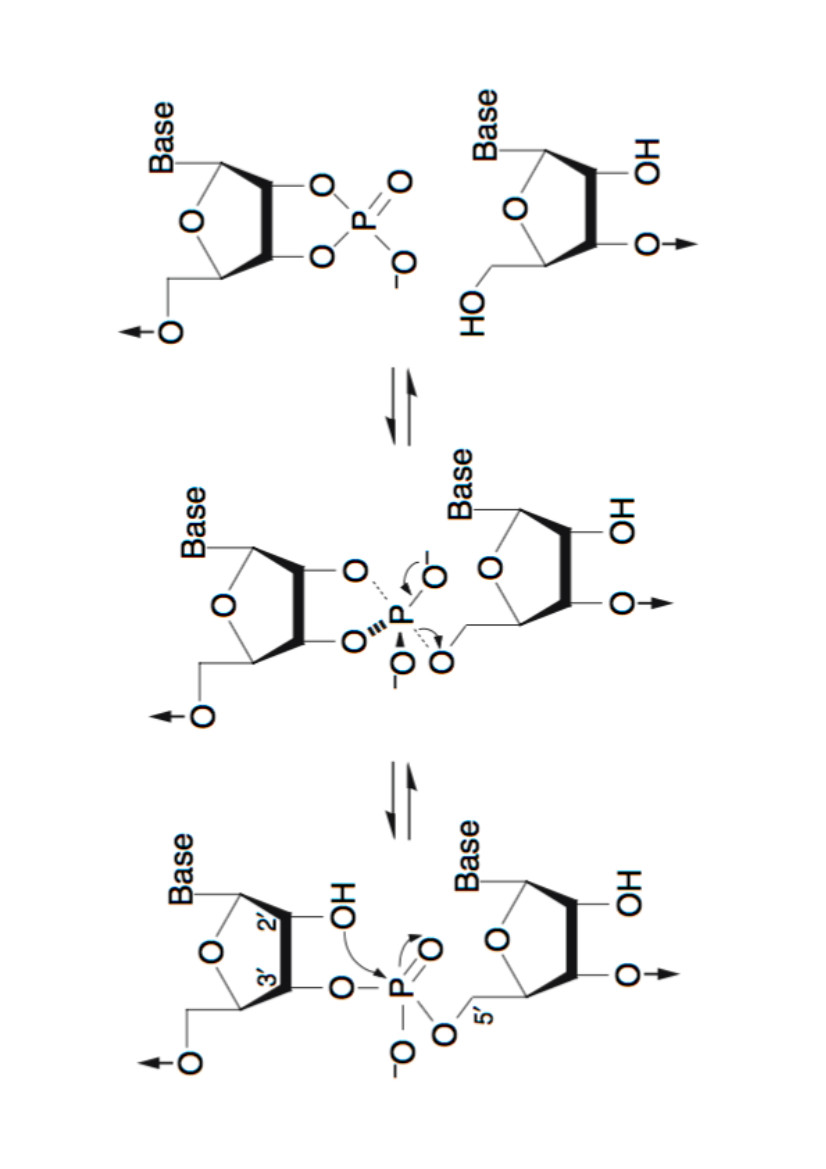
\includegraphics[scale=0.25,angle=270]{lectures/160527/pix/inline.jpg}

\textbf{Vorgehen:}
\begin{itemize}
\item Erstellen von zwei Proben des zu untersuchenden RNA-Moleküls
\item In einer Probe gewählten Ligand hinzugeben
\item beide Proben werden lange inkubiert $\rightarrow$ nucleophilic attack
\item Gelbild mittels Gelelektrophorese herstellen und Längen der RNA-Fragmente beider Proben vergleichend betrachten
\item gleiche Strukturen werden als Hintergrundrauschen (ligandenunabhängige) Cleavages betrachtet
\end{itemize}

\subsection{Chemisches Probing}
RNA-modifizierende Chemikalien sind \textbf{struktursensitiv} [1] und \textbf{sequenzunabhängig} \\
\begin{itemize}
\item[1] Es werden Chemikalien genutzt die entweder gepaarte oder ungepaarte Basen modifizieren
\item[2] Mechanismus zur Detektion der Modifikation
\end{itemize}

\subsubsection{SHAPE-Seq}
(\textbf{S}elective 2'-\textbf{h}ydroxylacetylation \textbf{a}nalyzed by \textbf{p}rimer \textbf{e}xtention \textbf{seq}uencing)

\begin{itemize}
\item 2'-OH ist reaktiver wenn die zugehörige Base ungebunden ist
\item genutzte Chemikalie: N-methylisatoic anhybdride
\item unter Abgabe von Kohlenstoffdioxid ($CO_2$) bindet ein Sauerstoffmolekül des NMIA an 2'-OH der RNA \\
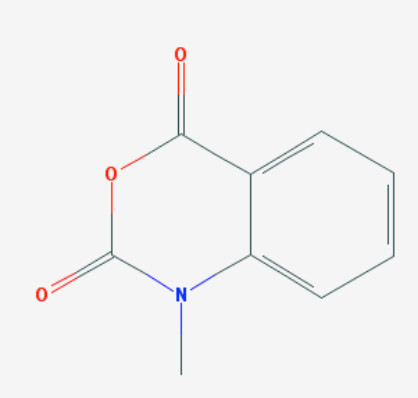
\includegraphics[scale=0.5]{lectures/160527/pix/NMIA.jpg} \\
(Quelle: $https://pubchem.ncbi.nlm.nih.gov/compound/N-Methylisatoic_anhydride$) \\

\item reverse Transkription: Die RNA wird mit DNA-Molekülen trankribiert.I m Anschluss werden die gewonnenen DNA-Fragmente sequenziert und als Library gespeichert
\item Da es auch zu zufälligen Abbruch bei der reversen Transkription kommen kann, wird ebenfalls eine negativ-Library erzeugt
\item Alignment der Reads an Transkriptom der RNA ($X_ij$, wobei i = Basenposition, j = Library)

\item Maximum-Likelihood-Model:

\begin{itemize}
\item $r_i = \dfrac{r_{i+}}{r_{i-}}$ $\rightarrow$ Datengrundlage
\item negativ-Library $\rightarrow$ Abbruchrate
\item simulierte Daten $m_i$ $\rightarrow$ Berechnung der positionsweisen Shape-Reaktivität 
\end{itemize}

\item[$\rightarrow$] Ermittlung der pseudo-Free-Energy

\begin{equation}
\Delta G_{Shape_i} = m * ln(\gamma_i * 1,0) + b
\end{equation}

\end{itemize}

m ... Anstieg des Bestrafungswertes \\
1,0 ... Pseudocount
b ... negativer Bonus der freien Energie für gepaarte Basen

\begin{equation}
M_{ij} = min
\begin{cases} 
M(i+1,j \\
min (M(i+1,k-1)*M(k+1,j)*e^{-\dfrac{E^{'}_{ij}}{kT}})
\end{cases}
\end{equation}

wobei:
\begin{equation}
E^{'}_{ij} = E_{ij} + \Delta G_{Shape_i} + \Delta G_{Shape_j}
\end{equation}

$E_{ij}$ ... Standard Energiemodell

\subsubsection{objective function approach}
\textbf{Hard constraints:} \\
$\rightarrow$ 3 Aussagen möglich: | = gepaart; . = ungepaart; X = unbekannt \\
\textbf{Soft constraints:} \\ 
$\rightarrow$ Wahrscheinlichkeit ob Base an Position Y gepaart ist oder nicht 

$\rightarrow$ Minimiere den Fehler F($\vec{E}$) \\
\begin{equation}
\vec{E} = \sum_{\mu} \dfrac{\varepsilon_{\mu}^{2}}{\tau^2} + \sum_{i = 0}^{n} \dfrac{1}{\sigma^2}(p_i(\vec{\varepsilon}) -q_i)^2
\end{equation} 

$\mu$ ... Strukturelemente
$\varepsilon_{\mu}$ ... Betrag der Stör-Energie eines Strukturelements\\
$\tau^2$ ... Varianz des Standardenergiemodells \\
$\sigma^2$ ... Varianz der Probingdaten \\
$p_i(\vec{\varepsilon})$ ... Wahrscheinlichkeit, dass i ungepaart ist unter Bedingung des Standardenergiemodells und der Störenergie

\subsubsection{Hydroxyl-Radikal Probing}
Hydroxyl-Radikale führen zum Bruch der RNA-Sequenz,wenn keine 3-D Interaktion stattfindet und keine Bindung an ein Protein vorliegt.\\
Nachteil: Sie sind nur kurzlebig in Lösung und müssen hergestellt werden

\subsubsection{DMS}
Di-Methylsulfat bindet an $CH_3$ von ungebundenen A bzw. C oder an eines der beiden, wenn sie das letzte Basenpaar einer Helix bilden oder wenn sie direkt neben einem GU-Basenpaar liegen. \\
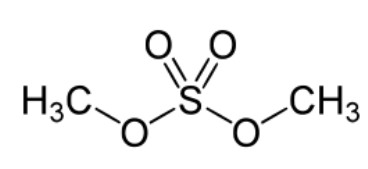
\includegraphics[scale=0.3]{lectures/160527/pix/Dimethylsulfat.jpg} \\

\subsubsection{CMCT}
(1-Cyclohexyl-(2-Morpholinoethyl)Carbodiimid Metho-p-Toluensulfonat) modifiziert vorwiegend ungepaartes Uridin und teilweise ungepaartes Guanin. \\
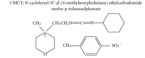
\includegraphics[scale=1]{lectures/160527/pix/CMCT.jpg} \\

\subsubsection{Kethoxal}
Kethoxal modifiziert ungepaartes Guanin \\
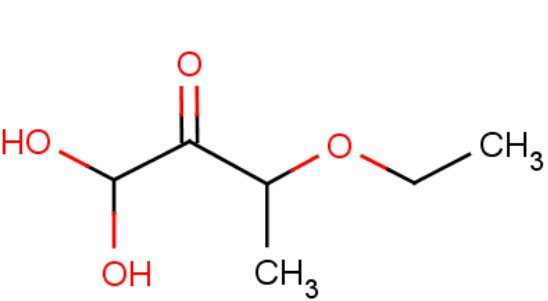
\includegraphics[scale=0.3]{lectures/160527/pix/Kethoxal.jpg}

\subsection{Nucleotide analoge interference mapping (NAIM)}
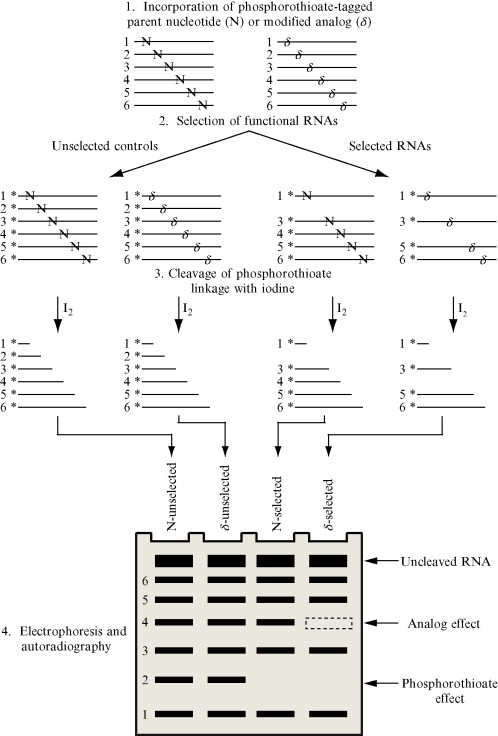
\includegraphics[scale=0.7]{lectures/160527/pix/NAIM.jpg} \\
(Quelle: http://www.sciencedirect.com/science/article/pii/S0076687909680010) \\
 
NAIM ist eine Erweiterung des Interferenz-Mappings mit Triphosphorsäure-Substitution
Untersucht, welche Basen funktional sind. Vorgehensweise:
\begin{itemize}
\item Nukleotide sind prinzipiell ohne funktionelle Gruppe
\item Nukleotide werden in vitro zufällig durch getaggede Analogika und getaggede normale Nukleotide während Transkription markiert
\item Annahme: Jedes Transkript hat nur ein getaggedes Nukleotid/Analogon
\item Auswahl der aktiven funktionalen RNAs und Erzeugung einer inaktiven Kontrollgruppe
\item Cleavage (Beschneiden) hinter der getaggeden Struktur durch Iod
\item Gelelektrophoresebild $\rightarrow$ gibt Aussage darüber welche durch Selektion sichtbar werden und welche durch Nukleotid-Einbau sichtbar sind
\end{itemize}

\newpage

\section{RNA structure probing}
\textbf{Bestimmung von:}
\begin{itemize}
\item Basenpaarung
\item Sekundärstruktur und Tertiärstruktur
\end{itemize}

\subsection{Inline-Probing}
inline-nucleophilic-attack: Wie in der Abbildung zu sehen kommt es zu strukturellen Änderungen der chemischen Konformation des RNA-Strangs an der Phosphatgruppe. Grund hierfür ist die Instabilität der Einzelsträngigen RNA, die bei Bindung eines Liganden an das Molekül zum Bruch ("Cleavage") führt oder eine rein zufällige Konformationsänderung des RNA-Moleküls. \\
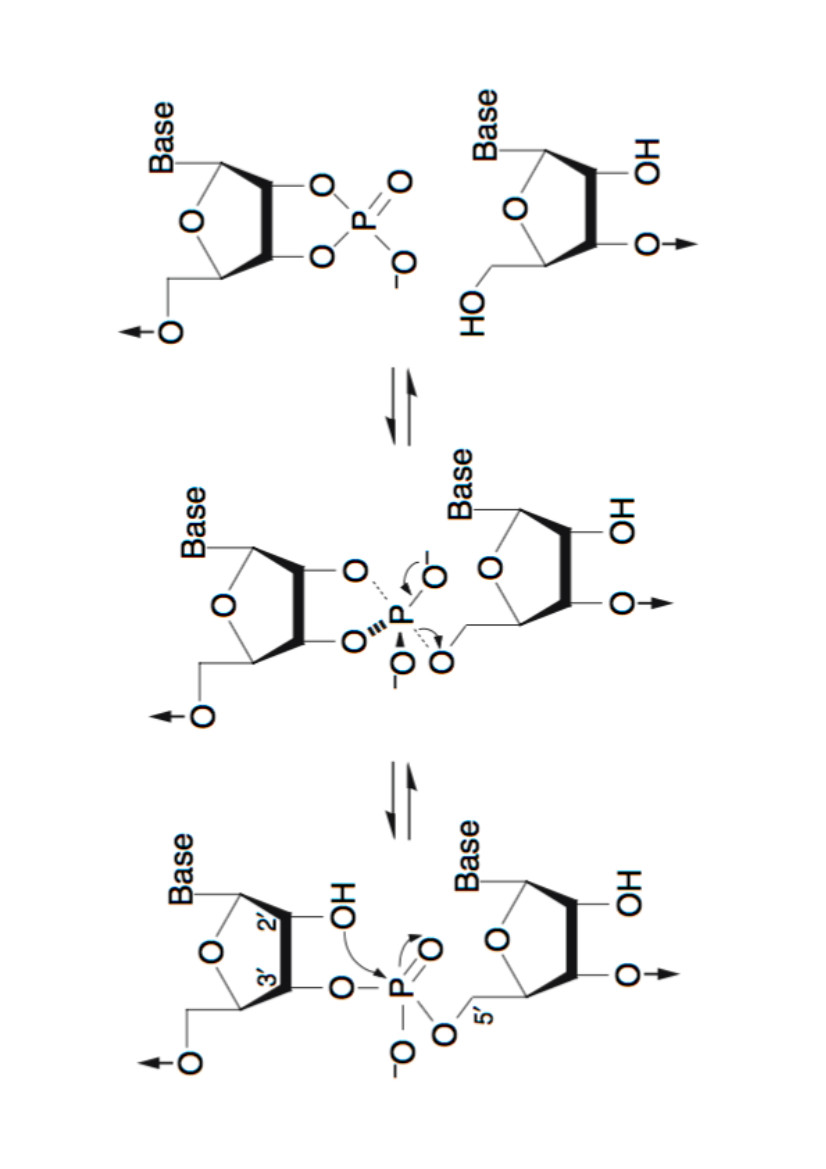
\includegraphics[scale=0.25,angle=270]{lectures/160527/pix/inline.jpg}

\textbf{Vorgehen:}
\begin{itemize}
\item Erstellen von zwei Proben des zu untersuchenden RNA-Moleküls
\item In einer Probe gewählten Ligand hinzugeben
\item beide Proben werden lange inkubiert $\rightarrow$ nucleophilic attack
\item Gelbild mittels Gelelektrophorese herstellen und Längen der RNA-Fragmente beider Proben vergleichend betrachten
\item gleiche Strukturen werden als Hintergrundrauschen (ligandenunabhängige) Cleavages betrachtet
\end{itemize}

\subsection{Chemisches Probing}
RNA-modifizierende Chemikalien sind \textbf{struktursensitiv} [1] und \textbf{sequenzunabhängig} \\
\begin{itemize}
\item[1] Es werden Chemikalien genutzt die entweder gepaarte oder ungepaarte Basen modifizieren
\item[2] Mechanismus zur Detektion der Modifikation
\end{itemize}

\subsubsection{SHAPE-Seq}
(\textbf{S}elective 2'-\textbf{h}ydroxylacetylation \textbf{a}nalyzed by \textbf{p}rimer \textbf{e}xtention \textbf{seq}uencing)

\begin{itemize}
\item 2'-OH ist reaktiver wenn die zugehörige Base ungebunden ist
\item genutzte Chemikalie: N-methylisatoic anhybdride
\item unter Abgabe von Kohlenstoffdioxid ($CO_2$) bindet ein Sauerstoffmolekül des NMIA an 2'-OH der RNA \\
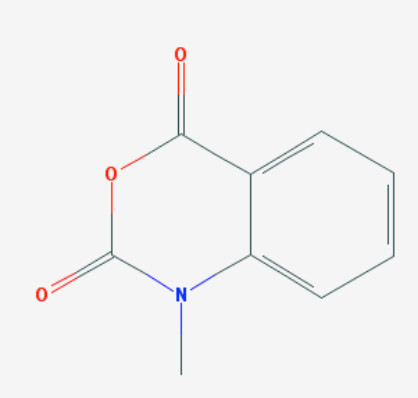
\includegraphics[scale=0.5]{lectures/160527/pix/NMIA.jpg} \\
(Quelle: $https://pubchem.ncbi.nlm.nih.gov/compound/N-Methylisatoic_anhydride$) \\

\item reverse Transkription: Die RNA wird mit DNA-Molekülen trankribiert.I m Anschluss werden die gewonnenen DNA-Fragmente sequenziert und als Library gespeichert
\item Da es auch zu zufälligen Abbruch bei der reversen Transkription kommen kann, wird ebenfalls eine negativ-Library erzeugt
\item Alignment der Reads an Transkriptom der RNA ($X_ij$, wobei i = Basenposition, j = Library)

\item Maximum-Likelihood-Model:

\begin{itemize}
\item $r_i = \dfrac{r_{i+}}{r_{i-}}$ $\rightarrow$ Datengrundlage
\item negativ-Library $\rightarrow$ Abbruchrate
\item simulierte Daten $m_i$ $\rightarrow$ Berechnung der positionsweisen Shape-Reaktivität 
\end{itemize}

\item[$\rightarrow$] Ermittlung der pseudo-Free-Energy

\begin{equation}
\Delta G_{Shape_i} = m * ln(\gamma_i * 1,0) + b
\end{equation}

\end{itemize}

m ... Anstieg des Bestrafungswertes \\
1,0 ... Pseudocount
b ... negativer Bonus der freien Energie für gepaarte Basen

\begin{equation}
M_{ij} = min
\begin{cases} 
M(i+1,j \\
min (M(i+1,k-1)*M(k+1,j)*e^{-\dfrac{E^{'}_{ij}}{kT}})
\end{cases}
\end{equation}

wobei:
\begin{equation}
E^{'}_{ij} = E_{ij} + \Delta G_{Shape_i} + \Delta G_{Shape_j}
\end{equation}

$E_{ij}$ ... Standard Energiemodell

\subsubsection{objective function approach}
\textbf{Hard constraints:} \\
$\rightarrow$ 3 Aussagen möglich: | = gepaart; . = ungepaart; X = unbekannt \\
\textbf{Soft constraints:} \\ 
$\rightarrow$ Wahrscheinlichkeit ob Base an Position Y gepaart ist oder nicht 

$\rightarrow$ Minimiere den Fehler F($\vec{E}$) \\
\begin{equation}
\vec{E} = \sum_{\mu} \dfrac{\varepsilon_{\mu}^{2}}{\tau^2} + \sum_{i = 0}^{n} \dfrac{1}{\sigma^2}(p_i(\vec{\varepsilon}) -q_i)^2
\end{equation} 

$\mu$ ... Strukturelemente
$\varepsilon_{\mu}$ ... Betrag der Stör-Energie eines Strukturelements\\
$\tau^2$ ... Varianz des Standardenergiemodells \\
$\sigma^2$ ... Varianz der Probingdaten \\
$p_i(\vec{\varepsilon})$ ... Wahrscheinlichkeit, dass i ungepaart ist unter Bedingung des Standardenergiemodells und der Störenergie

\subsubsection{Hydroxyl-Radikal Probing}
Hydroxyl-Radikale führen zum Bruch der RNA-Sequenz,wenn keine 3-D Interaktion stattfindet und keine Bindung an ein Protein vorliegt.\\
Nachteil: Sie sind nur kurzlebig in Lösung und müssen hergestellt werden

\subsubsection{DMS}
Di-Methylsulfat bindet an $CH_3$ von ungebundenen A bzw. C oder an eines der beiden, wenn sie das letzte Basenpaar einer Helix bilden oder wenn sie direkt neben einem GU-Basenpaar liegen. \\
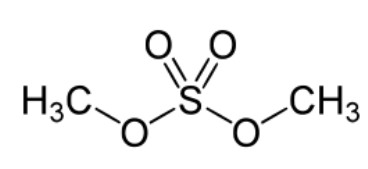
\includegraphics[scale=0.3]{lectures/160527/pix/Dimethylsulfat.jpg} \\

\subsubsection{CMCT}
(1-Cyclohexyl-(2-Morpholinoethyl)Carbodiimid Metho-p-Toluensulfonat) modifiziert vorwiegend ungepaartes Uridin und teilweise ungepaartes Guanin. \\
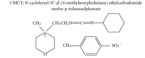
\includegraphics[scale=1]{lectures/160527/pix/CMCT.jpg} \\

\subsubsection{Kethoxal}
Kethoxal modifiziert ungepaartes Guanin \\
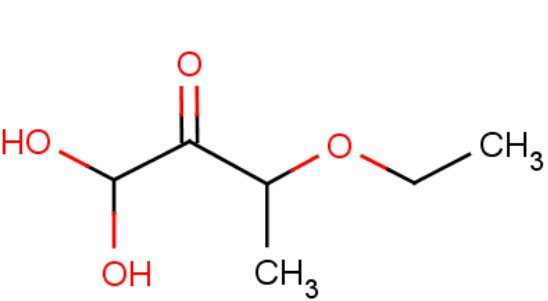
\includegraphics[scale=0.3]{lectures/160527/pix/Kethoxal.jpg}

\subsection{Nucleotide analoge interference mapping (NAIM)}
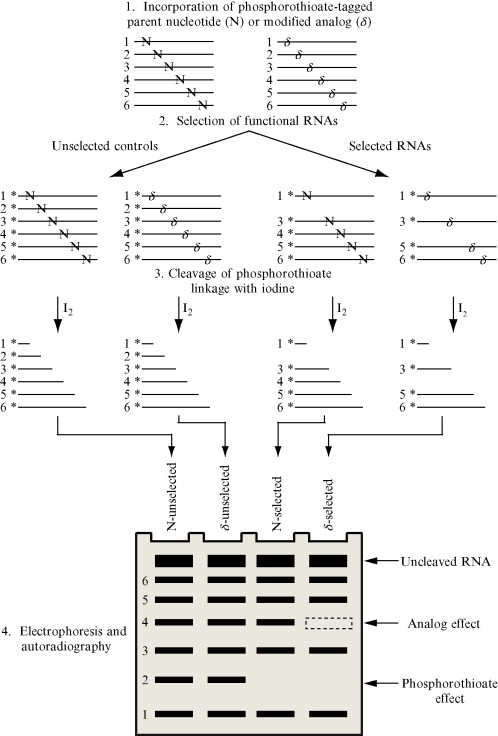
\includegraphics[scale=0.7]{lectures/160527/pix/NAIM.jpg} \\
(Quelle: http://www.sciencedirect.com/science/article/pii/S0076687909680010) \\
 
NAIM ist eine Erweiterung des Interferenz-Mappings mit Triphosphorsäure-Substitution
Untersucht, welche Basen funktional sind. Vorgehensweise:
\begin{itemize}
\item Nukleotide sind prinzipiell ohne funktionelle Gruppe
\item Nukleotide werden in vitro zufällig durch getaggede Analogika und getaggede normale Nukleotide während Transkription markiert
\item Annahme: Jedes Transkript hat nur ein getaggedes Nukleotid/Analogon
\item Auswahl der aktiven funktionalen RNAs und Erzeugung einer inaktiven Kontrollgruppe
\item Cleavage (Beschneiden) hinter der getaggeden Struktur durch Iod
\item Gelelektrophoresebild $\rightarrow$ gibt Aussage darüber welche durch Selektion sichtbar werden und welche durch Nukleotid-Einbau sichtbar sind
\end{itemize}

\newpage

\section{RNA structure probing}
\textbf{Bestimmung von:}
\begin{itemize}
\item Basenpaarung
\item Sekundärstruktur und Tertiärstruktur
\end{itemize}

\subsection{Inline-Probing}
inline-nucleophilic-attack: Wie in der Abbildung zu sehen kommt es zu strukturellen Änderungen der chemischen Konformation des RNA-Strangs an der Phosphatgruppe. Grund hierfür ist die Instabilität der Einzelsträngigen RNA, die bei Bindung eines Liganden an das Molekül zum Bruch ("Cleavage") führt oder eine rein zufällige Konformationsänderung des RNA-Moleküls. \\
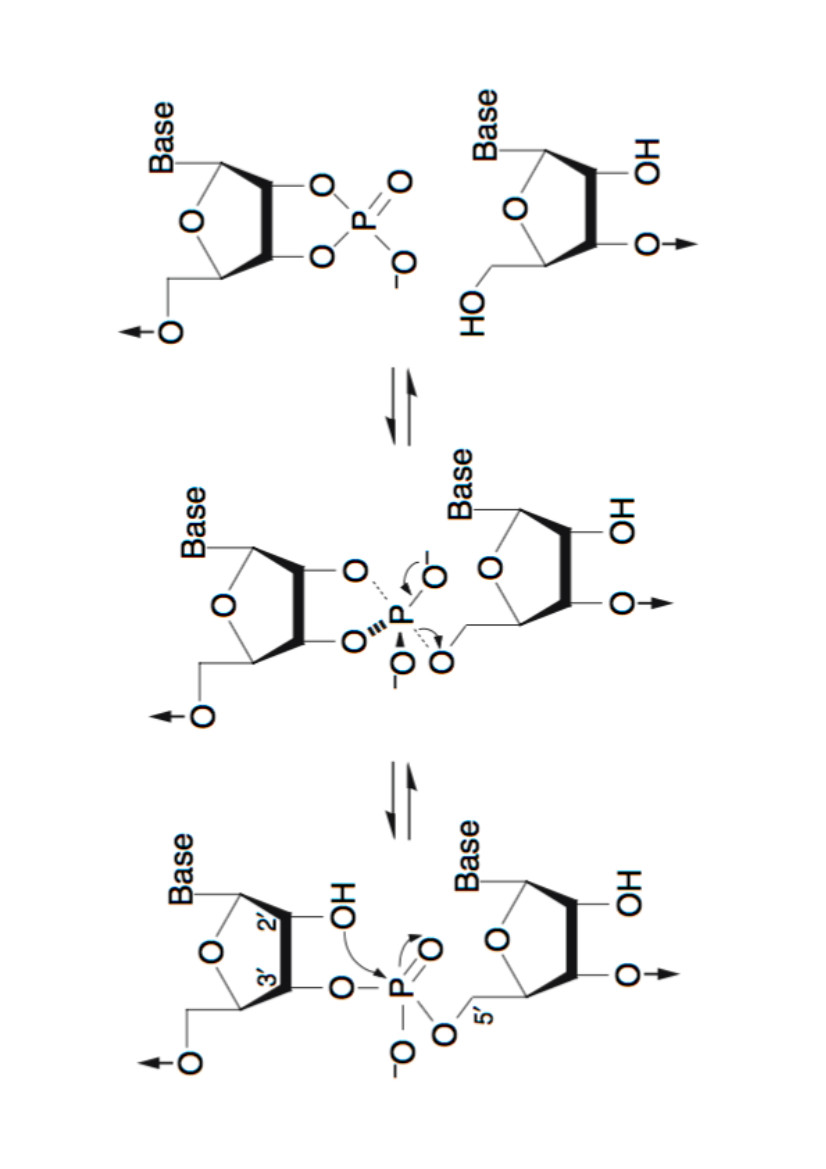
\includegraphics[scale=0.25,angle=270]{lectures/160527/pix/inline.jpg}

\textbf{Vorgehen:}
\begin{itemize}
\item Erstellen von zwei Proben des zu untersuchenden RNA-Moleküls
\item In einer Probe gewählten Ligand hinzugeben
\item beide Proben werden lange inkubiert $\rightarrow$ nucleophilic attack
\item Gelbild mittels Gelelektrophorese herstellen und Längen der RNA-Fragmente beider Proben vergleichend betrachten
\item gleiche Strukturen werden als Hintergrundrauschen (ligandenunabhängige) Cleavages betrachtet
\end{itemize}

\subsection{Chemisches Probing}
RNA-modifizierende Chemikalien sind \textbf{struktursensitiv} [1] und \textbf{sequenzunabhängig} \\
\begin{itemize}
\item[1] Es werden Chemikalien genutzt die entweder gepaarte oder ungepaarte Basen modifizieren
\item[2] Mechanismus zur Detektion der Modifikation
\end{itemize}

\subsubsection{SHAPE-Seq}
(\textbf{S}elective 2'-\textbf{h}ydroxylacetylation \textbf{a}nalyzed by \textbf{p}rimer \textbf{e}xtention \textbf{seq}uencing)

\begin{itemize}
\item 2'-OH ist reaktiver wenn die zugehörige Base ungebunden ist
\item genutzte Chemikalie: N-methylisatoic anhybdride
\item unter Abgabe von Kohlenstoffdioxid ($CO_2$) bindet ein Sauerstoffmolekül des NMIA an 2'-OH der RNA \\
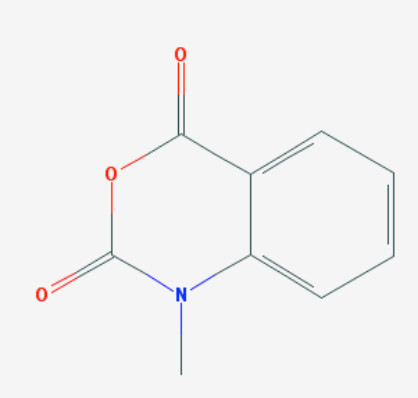
\includegraphics[scale=0.5]{lectures/160527/pix/NMIA.jpg} \\
(Quelle: $https://pubchem.ncbi.nlm.nih.gov/compound/N-Methylisatoic_anhydride$) \\

\item reverse Transkription: Die RNA wird mit DNA-Molekülen trankribiert.I m Anschluss werden die gewonnenen DNA-Fragmente sequenziert und als Library gespeichert
\item Da es auch zu zufälligen Abbruch bei der reversen Transkription kommen kann, wird ebenfalls eine negativ-Library erzeugt
\item Alignment der Reads an Transkriptom der RNA ($X_ij$, wobei i = Basenposition, j = Library)

\item Maximum-Likelihood-Model:

\begin{itemize}
\item $r_i = \dfrac{r_{i+}}{r_{i-}}$ $\rightarrow$ Datengrundlage
\item negativ-Library $\rightarrow$ Abbruchrate
\item simulierte Daten $m_i$ $\rightarrow$ Berechnung der positionsweisen Shape-Reaktivität 
\end{itemize}

\item[$\rightarrow$] Ermittlung der pseudo-Free-Energy

\begin{equation}
\Delta G_{Shape_i} = m * ln(\gamma_i * 1,0) + b
\end{equation}

\end{itemize}

m ... Anstieg des Bestrafungswertes \\
1,0 ... Pseudocount
b ... negativer Bonus der freien Energie für gepaarte Basen

\begin{equation}
M_{ij} = min
\begin{cases} 
M(i+1,j \\
min (M(i+1,k-1)*M(k+1,j)*e^{-\dfrac{E^{'}_{ij}}{kT}})
\end{cases}
\end{equation}

wobei:
\begin{equation}
E^{'}_{ij} = E_{ij} + \Delta G_{Shape_i} + \Delta G_{Shape_j}
\end{equation}

$E_{ij}$ ... Standard Energiemodell

\subsubsection{objective function approach}
\textbf{Hard constraints:} \\
$\rightarrow$ 3 Aussagen möglich: | = gepaart; . = ungepaart; X = unbekannt \\
\textbf{Soft constraints:} \\ 
$\rightarrow$ Wahrscheinlichkeit ob Base an Position Y gepaart ist oder nicht 

$\rightarrow$ Minimiere den Fehler F($\vec{E}$) \\
\begin{equation}
\vec{E} = \sum_{\mu} \dfrac{\varepsilon_{\mu}^{2}}{\tau^2} + \sum_{i = 0}^{n} \dfrac{1}{\sigma^2}(p_i(\vec{\varepsilon}) -q_i)^2
\end{equation} 

$\mu$ ... Strukturelemente
$\varepsilon_{\mu}$ ... Betrag der Stör-Energie eines Strukturelements\\
$\tau^2$ ... Varianz des Standardenergiemodells \\
$\sigma^2$ ... Varianz der Probingdaten \\
$p_i(\vec{\varepsilon})$ ... Wahrscheinlichkeit, dass i ungepaart ist unter Bedingung des Standardenergiemodells und der Störenergie

\subsubsection{Hydroxyl-Radikal Probing}
Hydroxyl-Radikale führen zum Bruch der RNA-Sequenz,wenn keine 3-D Interaktion stattfindet und keine Bindung an ein Protein vorliegt.\\
Nachteil: Sie sind nur kurzlebig in Lösung und müssen hergestellt werden

\subsubsection{DMS}
Di-Methylsulfat bindet an $CH_3$ von ungebundenen A bzw. C oder an eines der beiden, wenn sie das letzte Basenpaar einer Helix bilden oder wenn sie direkt neben einem GU-Basenpaar liegen. \\
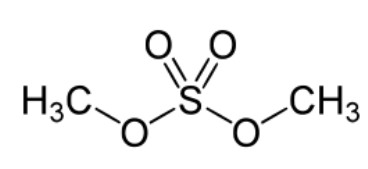
\includegraphics[scale=0.3]{lectures/160527/pix/Dimethylsulfat.jpg} \\

\subsubsection{CMCT}
(1-Cyclohexyl-(2-Morpholinoethyl)Carbodiimid Metho-p-Toluensulfonat) modifiziert vorwiegend ungepaartes Uridin und teilweise ungepaartes Guanin. \\
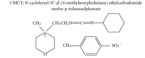
\includegraphics[scale=1]{lectures/160527/pix/CMCT.jpg} \\

\subsubsection{Kethoxal}
Kethoxal modifiziert ungepaartes Guanin \\
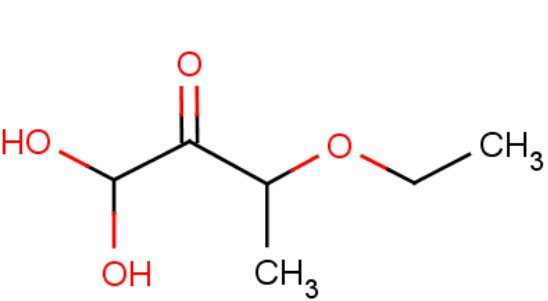
\includegraphics[scale=0.3]{lectures/160527/pix/Kethoxal.jpg}

\subsection{Nucleotide analoge interference mapping (NAIM)}
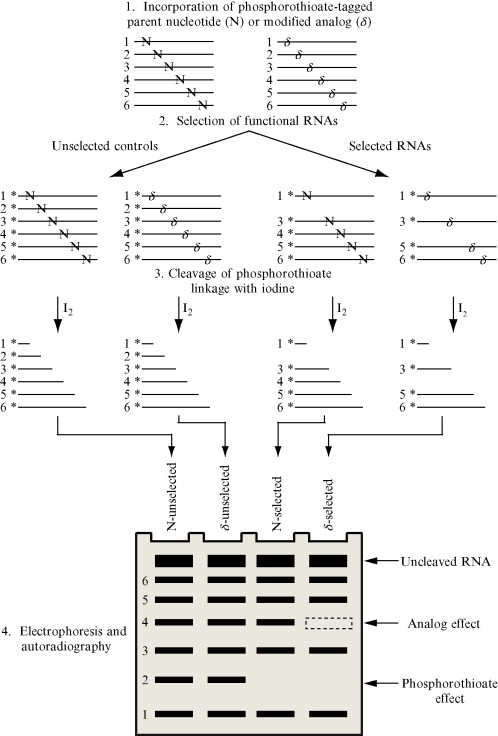
\includegraphics[scale=0.7]{lectures/160527/pix/NAIM.jpg} \\
(Quelle: http://www.sciencedirect.com/science/article/pii/S0076687909680010) \\
 
NAIM ist eine Erweiterung des Interferenz-Mappings mit Triphosphorsäure-Substitution
Untersucht, welche Basen funktional sind. Vorgehensweise:
\begin{itemize}
\item Nukleotide sind prinzipiell ohne funktionelle Gruppe
\item Nukleotide werden in vitro zufällig durch getaggede Analogika und getaggede normale Nukleotide während Transkription markiert
\item Annahme: Jedes Transkript hat nur ein getaggedes Nukleotid/Analogon
\item Auswahl der aktiven funktionalen RNAs und Erzeugung einer inaktiven Kontrollgruppe
\item Cleavage (Beschneiden) hinter der getaggeden Struktur durch Iod
\item Gelelektrophoresebild $\rightarrow$ gibt Aussage darüber welche durch Selektion sichtbar werden und welche durch Nukleotid-Einbau sichtbar sind
\end{itemize}

\newpage

\section{RNA structure probing}
\textbf{Bestimmung von:}
\begin{itemize}
\item Basenpaarung
\item Sekundärstruktur und Tertiärstruktur
\end{itemize}

\subsection{Inline-Probing}
inline-nucleophilic-attack: Wie in der Abbildung zu sehen kommt es zu strukturellen Änderungen der chemischen Konformation des RNA-Strangs an der Phosphatgruppe. Grund hierfür ist die Instabilität der Einzelsträngigen RNA, die bei Bindung eines Liganden an das Molekül zum Bruch ("Cleavage") führt oder eine rein zufällige Konformationsänderung des RNA-Moleküls. \\
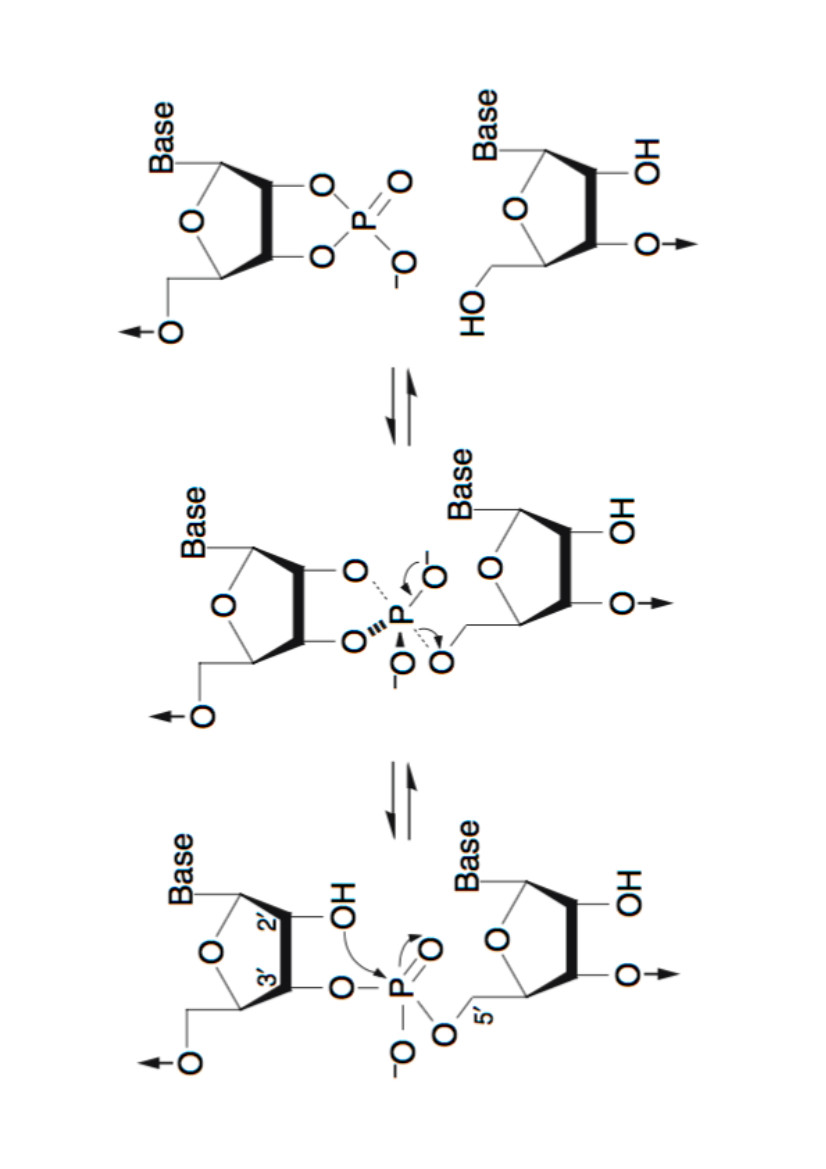
\includegraphics[scale=0.25,angle=270]{lectures/160527/pix/inline.jpg}

\textbf{Vorgehen:}
\begin{itemize}
\item Erstellen von zwei Proben des zu untersuchenden RNA-Moleküls
\item In einer Probe gewählten Ligand hinzugeben
\item beide Proben werden lange inkubiert $\rightarrow$ nucleophilic attack
\item Gelbild mittels Gelelektrophorese herstellen und Längen der RNA-Fragmente beider Proben vergleichend betrachten
\item gleiche Strukturen werden als Hintergrundrauschen (ligandenunabhängige) Cleavages betrachtet
\end{itemize}

\subsection{Chemisches Probing}
RNA-modifizierende Chemikalien sind \textbf{struktursensitiv} [1] und \textbf{sequenzunabhängig} \\
\begin{itemize}
\item[1] Es werden Chemikalien genutzt die entweder gepaarte oder ungepaarte Basen modifizieren
\item[2] Mechanismus zur Detektion der Modifikation
\end{itemize}

\subsubsection{SHAPE-Seq}
(\textbf{S}elective 2'-\textbf{h}ydroxylacetylation \textbf{a}nalyzed by \textbf{p}rimer \textbf{e}xtention \textbf{seq}uencing)

\begin{itemize}
\item 2'-OH ist reaktiver wenn die zugehörige Base ungebunden ist
\item genutzte Chemikalie: N-methylisatoic anhybdride
\item unter Abgabe von Kohlenstoffdioxid ($CO_2$) bindet ein Sauerstoffmolekül des NMIA an 2'-OH der RNA \\
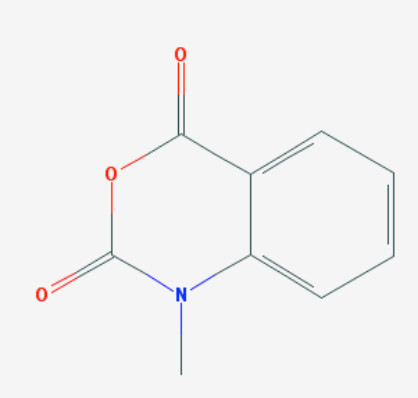
\includegraphics[scale=0.5]{lectures/160527/pix/NMIA.jpg} \\
(Quelle: $https://pubchem.ncbi.nlm.nih.gov/compound/N-Methylisatoic_anhydride$) \\

\item reverse Transkription: Die RNA wird mit DNA-Molekülen trankribiert.I m Anschluss werden die gewonnenen DNA-Fragmente sequenziert und als Library gespeichert
\item Da es auch zu zufälligen Abbruch bei der reversen Transkription kommen kann, wird ebenfalls eine negativ-Library erzeugt
\item Alignment der Reads an Transkriptom der RNA ($X_ij$, wobei i = Basenposition, j = Library)

\item Maximum-Likelihood-Model:

\begin{itemize}
\item $r_i = \dfrac{r_{i+}}{r_{i-}}$ $\rightarrow$ Datengrundlage
\item negativ-Library $\rightarrow$ Abbruchrate
\item simulierte Daten $m_i$ $\rightarrow$ Berechnung der positionsweisen Shape-Reaktivität 
\end{itemize}

\item[$\rightarrow$] Ermittlung der pseudo-Free-Energy

\begin{equation}
\Delta G_{Shape_i} = m * ln(\gamma_i * 1,0) + b
\end{equation}

\end{itemize}

m ... Anstieg des Bestrafungswertes \\
1,0 ... Pseudocount
b ... negativer Bonus der freien Energie für gepaarte Basen

\begin{equation}
M_{ij} = min
\begin{cases} 
M(i+1,j \\
min (M(i+1,k-1)*M(k+1,j)*e^{-\dfrac{E^{'}_{ij}}{kT}})
\end{cases}
\end{equation}

wobei:
\begin{equation}
E^{'}_{ij} = E_{ij} + \Delta G_{Shape_i} + \Delta G_{Shape_j}
\end{equation}

$E_{ij}$ ... Standard Energiemodell

\subsubsection{objective function approach}
\textbf{Hard constraints:} \\
$\rightarrow$ 3 Aussagen möglich: | = gepaart; . = ungepaart; X = unbekannt \\
\textbf{Soft constraints:} \\ 
$\rightarrow$ Wahrscheinlichkeit ob Base an Position Y gepaart ist oder nicht 

$\rightarrow$ Minimiere den Fehler F($\vec{E}$) \\
\begin{equation}
\vec{E} = \sum_{\mu} \dfrac{\varepsilon_{\mu}^{2}}{\tau^2} + \sum_{i = 0}^{n} \dfrac{1}{\sigma^2}(p_i(\vec{\varepsilon}) -q_i)^2
\end{equation} 

$\mu$ ... Strukturelemente
$\varepsilon_{\mu}$ ... Betrag der Stör-Energie eines Strukturelements\\
$\tau^2$ ... Varianz des Standardenergiemodells \\
$\sigma^2$ ... Varianz der Probingdaten \\
$p_i(\vec{\varepsilon})$ ... Wahrscheinlichkeit, dass i ungepaart ist unter Bedingung des Standardenergiemodells und der Störenergie

\subsubsection{Hydroxyl-Radikal Probing}
Hydroxyl-Radikale führen zum Bruch der RNA-Sequenz,wenn keine 3-D Interaktion stattfindet und keine Bindung an ein Protein vorliegt.\\
Nachteil: Sie sind nur kurzlebig in Lösung und müssen hergestellt werden

\subsubsection{DMS}
Di-Methylsulfat bindet an $CH_3$ von ungebundenen A bzw. C oder an eines der beiden, wenn sie das letzte Basenpaar einer Helix bilden oder wenn sie direkt neben einem GU-Basenpaar liegen. \\
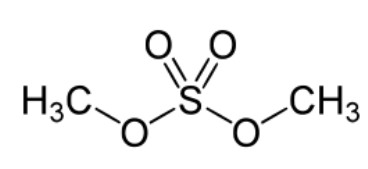
\includegraphics[scale=0.3]{lectures/160527/pix/Dimethylsulfat.jpg} \\

\subsubsection{CMCT}
(1-Cyclohexyl-(2-Morpholinoethyl)Carbodiimid Metho-p-Toluensulfonat) modifiziert vorwiegend ungepaartes Uridin und teilweise ungepaartes Guanin. \\
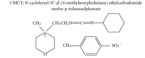
\includegraphics[scale=1]{lectures/160527/pix/CMCT.jpg} \\

\subsubsection{Kethoxal}
Kethoxal modifiziert ungepaartes Guanin \\
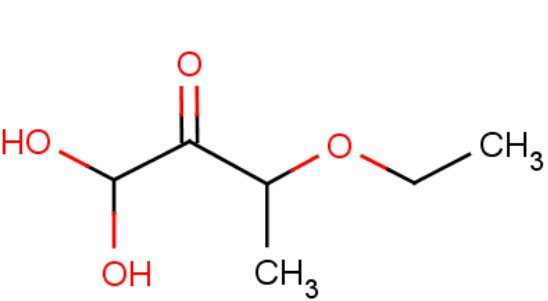
\includegraphics[scale=0.3]{lectures/160527/pix/Kethoxal.jpg}

\subsection{Nucleotide analoge interference mapping (NAIM)}
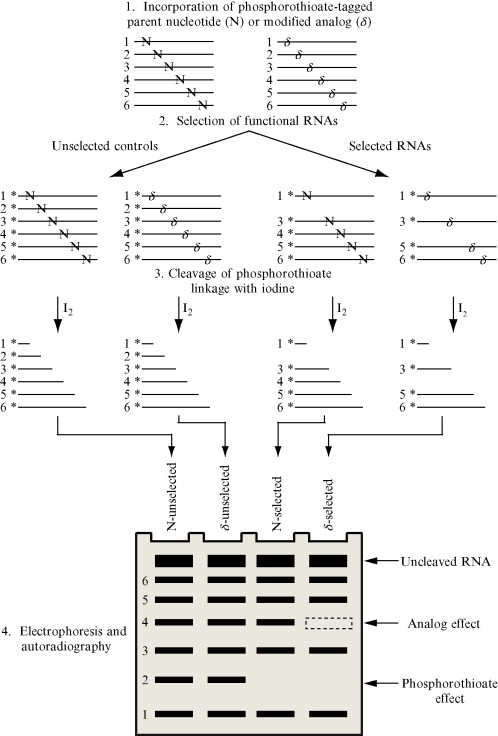
\includegraphics[scale=0.7]{lectures/160527/pix/NAIM.jpg} \\
(Quelle: http://www.sciencedirect.com/science/article/pii/S0076687909680010) \\
 
NAIM ist eine Erweiterung des Interferenz-Mappings mit Triphosphorsäure-Substitution
Untersucht, welche Basen funktional sind. Vorgehensweise:
\begin{itemize}
\item Nukleotide sind prinzipiell ohne funktionelle Gruppe
\item Nukleotide werden in vitro zufällig durch getaggede Analogika und getaggede normale Nukleotide während Transkription markiert
\item Annahme: Jedes Transkript hat nur ein getaggedes Nukleotid/Analogon
\item Auswahl der aktiven funktionalen RNAs und Erzeugung einer inaktiven Kontrollgruppe
\item Cleavage (Beschneiden) hinter der getaggeden Struktur durch Iod
\item Gelelektrophoresebild $\rightarrow$ gibt Aussage darüber welche durch Selektion sichtbar werden und welche durch Nukleotid-Einbau sichtbar sind
\end{itemize}

\newpage

\section{RNA structure probing}
\textbf{Bestimmung von:}
\begin{itemize}
\item Basenpaarung
\item Sekundärstruktur und Tertiärstruktur
\end{itemize}

\subsection{Inline-Probing}
inline-nucleophilic-attack: Wie in der Abbildung zu sehen kommt es zu strukturellen Änderungen der chemischen Konformation des RNA-Strangs an der Phosphatgruppe. Grund hierfür ist die Instabilität der Einzelsträngigen RNA, die bei Bindung eines Liganden an das Molekül zum Bruch ("Cleavage") führt oder eine rein zufällige Konformationsänderung des RNA-Moleküls. \\
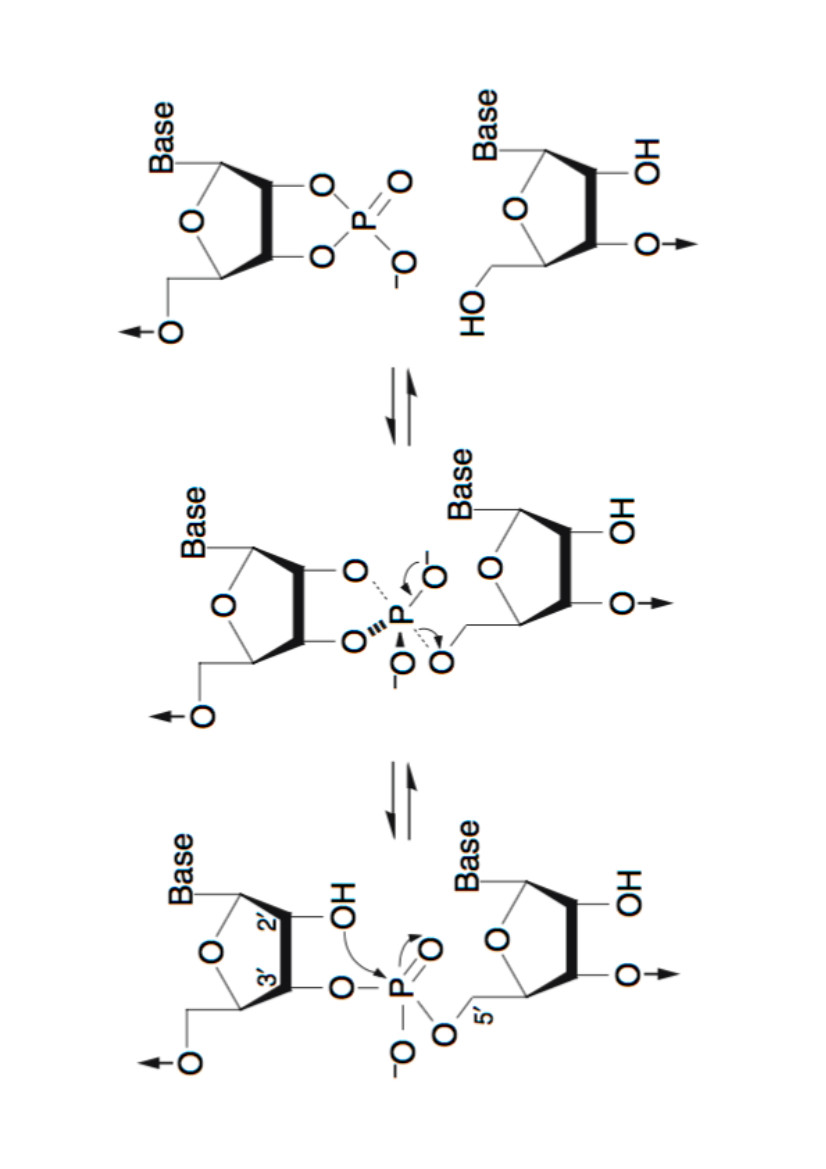
\includegraphics[scale=0.25,angle=270]{lectures/160527/pix/inline.jpg}

\textbf{Vorgehen:}
\begin{itemize}
\item Erstellen von zwei Proben des zu untersuchenden RNA-Moleküls
\item In einer Probe gewählten Ligand hinzugeben
\item beide Proben werden lange inkubiert $\rightarrow$ nucleophilic attack
\item Gelbild mittels Gelelektrophorese herstellen und Längen der RNA-Fragmente beider Proben vergleichend betrachten
\item gleiche Strukturen werden als Hintergrundrauschen (ligandenunabhängige) Cleavages betrachtet
\end{itemize}

\subsection{Chemisches Probing}
RNA-modifizierende Chemikalien sind \textbf{struktursensitiv} [1] und \textbf{sequenzunabhängig} \\
\begin{itemize}
\item[1] Es werden Chemikalien genutzt die entweder gepaarte oder ungepaarte Basen modifizieren
\item[2] Mechanismus zur Detektion der Modifikation
\end{itemize}

\subsubsection{SHAPE-Seq}
(\textbf{S}elective 2'-\textbf{h}ydroxylacetylation \textbf{a}nalyzed by \textbf{p}rimer \textbf{e}xtention \textbf{seq}uencing)

\begin{itemize}
\item 2'-OH ist reaktiver wenn die zugehörige Base ungebunden ist
\item genutzte Chemikalie: N-methylisatoic anhybdride
\item unter Abgabe von Kohlenstoffdioxid ($CO_2$) bindet ein Sauerstoffmolekül des NMIA an 2'-OH der RNA \\
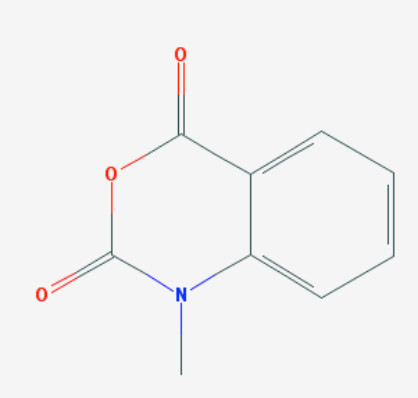
\includegraphics[scale=0.5]{lectures/160527/pix/NMIA.jpg} \\
(Quelle: $https://pubchem.ncbi.nlm.nih.gov/compound/N-Methylisatoic_anhydride$) \\

\item reverse Transkription: Die RNA wird mit DNA-Molekülen trankribiert.I m Anschluss werden die gewonnenen DNA-Fragmente sequenziert und als Library gespeichert
\item Da es auch zu zufälligen Abbruch bei der reversen Transkription kommen kann, wird ebenfalls eine negativ-Library erzeugt
\item Alignment der Reads an Transkriptom der RNA ($X_ij$, wobei i = Basenposition, j = Library)

\item Maximum-Likelihood-Model:

\begin{itemize}
\item $r_i = \dfrac{r_{i+}}{r_{i-}}$ $\rightarrow$ Datengrundlage
\item negativ-Library $\rightarrow$ Abbruchrate
\item simulierte Daten $m_i$ $\rightarrow$ Berechnung der positionsweisen Shape-Reaktivität 
\end{itemize}

\item[$\rightarrow$] Ermittlung der pseudo-Free-Energy

\begin{equation}
\Delta G_{Shape_i} = m * ln(\gamma_i * 1,0) + b
\end{equation}

\end{itemize}

m ... Anstieg des Bestrafungswertes \\
1,0 ... Pseudocount
b ... negativer Bonus der freien Energie für gepaarte Basen

\begin{equation}
M_{ij} = min
\begin{cases} 
M(i+1,j \\
min (M(i+1,k-1)*M(k+1,j)*e^{-\dfrac{E^{'}_{ij}}{kT}})
\end{cases}
\end{equation}

wobei:
\begin{equation}
E^{'}_{ij} = E_{ij} + \Delta G_{Shape_i} + \Delta G_{Shape_j}
\end{equation}

$E_{ij}$ ... Standard Energiemodell

\subsubsection{objective function approach}
\textbf{Hard constraints:} \\
$\rightarrow$ 3 Aussagen möglich: | = gepaart; . = ungepaart; X = unbekannt \\
\textbf{Soft constraints:} \\ 
$\rightarrow$ Wahrscheinlichkeit ob Base an Position Y gepaart ist oder nicht 

$\rightarrow$ Minimiere den Fehler F($\vec{E}$) \\
\begin{equation}
\vec{E} = \sum_{\mu} \dfrac{\varepsilon_{\mu}^{2}}{\tau^2} + \sum_{i = 0}^{n} \dfrac{1}{\sigma^2}(p_i(\vec{\varepsilon}) -q_i)^2
\end{equation} 

$\mu$ ... Strukturelemente
$\varepsilon_{\mu}$ ... Betrag der Stör-Energie eines Strukturelements\\
$\tau^2$ ... Varianz des Standardenergiemodells \\
$\sigma^2$ ... Varianz der Probingdaten \\
$p_i(\vec{\varepsilon})$ ... Wahrscheinlichkeit, dass i ungepaart ist unter Bedingung des Standardenergiemodells und der Störenergie

\subsubsection{Hydroxyl-Radikal Probing}
Hydroxyl-Radikale führen zum Bruch der RNA-Sequenz,wenn keine 3-D Interaktion stattfindet und keine Bindung an ein Protein vorliegt.\\
Nachteil: Sie sind nur kurzlebig in Lösung und müssen hergestellt werden

\subsubsection{DMS}
Di-Methylsulfat bindet an $CH_3$ von ungebundenen A bzw. C oder an eines der beiden, wenn sie das letzte Basenpaar einer Helix bilden oder wenn sie direkt neben einem GU-Basenpaar liegen. \\
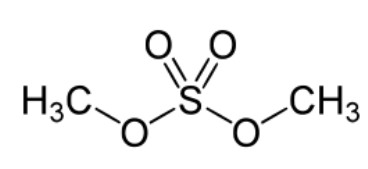
\includegraphics[scale=0.3]{lectures/160527/pix/Dimethylsulfat.jpg} \\

\subsubsection{CMCT}
(1-Cyclohexyl-(2-Morpholinoethyl)Carbodiimid Metho-p-Toluensulfonat) modifiziert vorwiegend ungepaartes Uridin und teilweise ungepaartes Guanin. \\
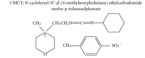
\includegraphics[scale=1]{lectures/160527/pix/CMCT.jpg} \\

\subsubsection{Kethoxal}
Kethoxal modifiziert ungepaartes Guanin \\
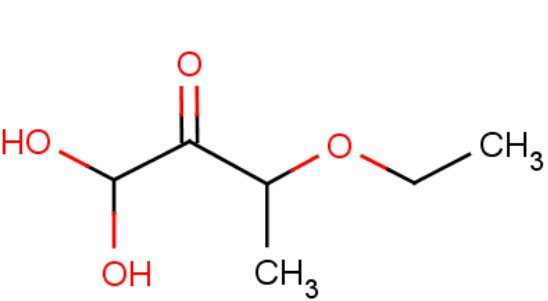
\includegraphics[scale=0.3]{lectures/160527/pix/Kethoxal.jpg}

\subsection{Nucleotide analoge interference mapping (NAIM)}
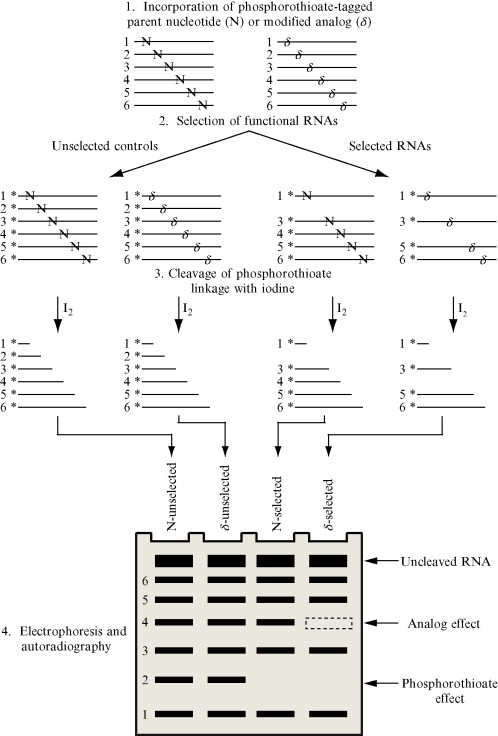
\includegraphics[scale=0.7]{lectures/160527/pix/NAIM.jpg} \\
(Quelle: http://www.sciencedirect.com/science/article/pii/S0076687909680010) \\
 
NAIM ist eine Erweiterung des Interferenz-Mappings mit Triphosphorsäure-Substitution
Untersucht, welche Basen funktional sind. Vorgehensweise:
\begin{itemize}
\item Nukleotide sind prinzipiell ohne funktionelle Gruppe
\item Nukleotide werden in vitro zufällig durch getaggede Analogika und getaggede normale Nukleotide während Transkription markiert
\item Annahme: Jedes Transkript hat nur ein getaggedes Nukleotid/Analogon
\item Auswahl der aktiven funktionalen RNAs und Erzeugung einer inaktiven Kontrollgruppe
\item Cleavage (Beschneiden) hinter der getaggeden Struktur durch Iod
\item Gelelektrophoresebild $\rightarrow$ gibt Aussage darüber welche durch Selektion sichtbar werden und welche durch Nukleotid-Einbau sichtbar sind
\end{itemize}

\newpage

\section{RNA structure probing}
\textbf{Bestimmung von:}
\begin{itemize}
\item Basenpaarung
\item Sekundärstruktur und Tertiärstruktur
\end{itemize}

\subsection{Inline-Probing}
inline-nucleophilic-attack: Wie in der Abbildung zu sehen kommt es zu strukturellen Änderungen der chemischen Konformation des RNA-Strangs an der Phosphatgruppe. Grund hierfür ist die Instabilität der Einzelsträngigen RNA, die bei Bindung eines Liganden an das Molekül zum Bruch ("Cleavage") führt oder eine rein zufällige Konformationsänderung des RNA-Moleküls. \\
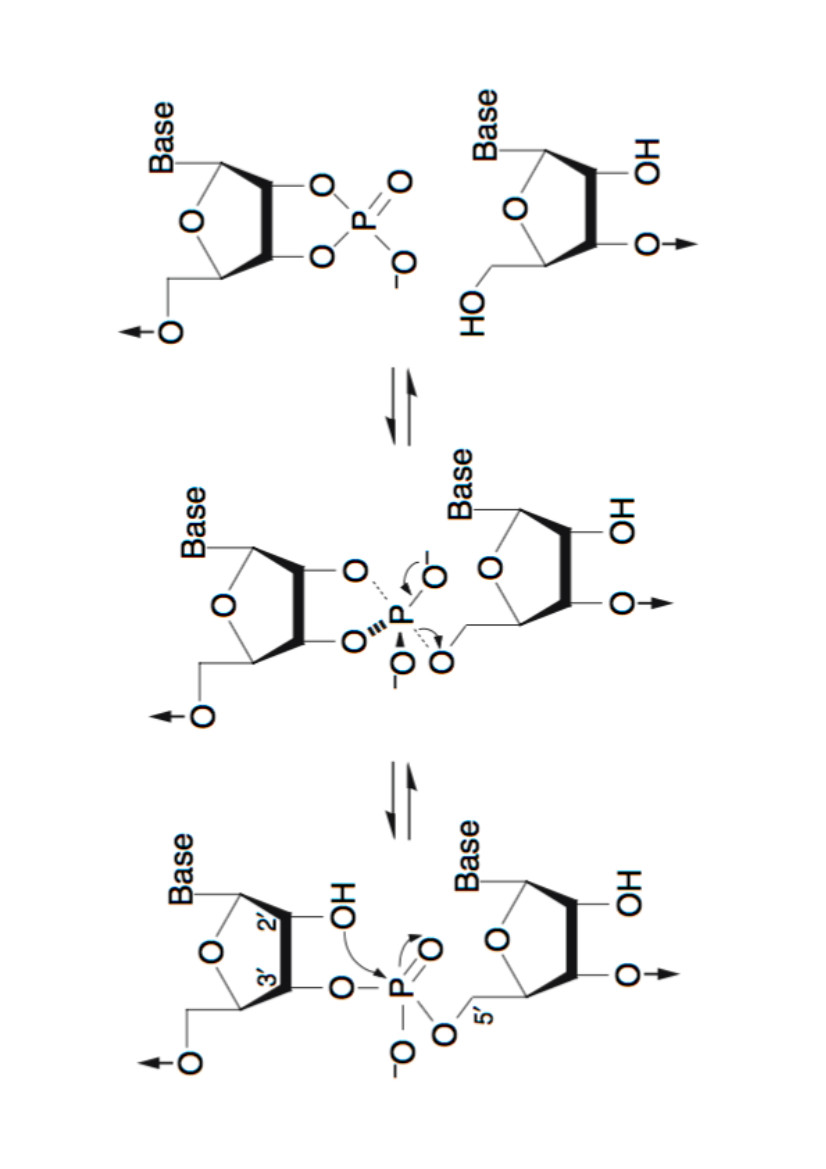
\includegraphics[scale=0.25,angle=270]{lectures/160527/pix/inline.jpg}

\textbf{Vorgehen:}
\begin{itemize}
\item Erstellen von zwei Proben des zu untersuchenden RNA-Moleküls
\item In einer Probe gewählten Ligand hinzugeben
\item beide Proben werden lange inkubiert $\rightarrow$ nucleophilic attack
\item Gelbild mittels Gelelektrophorese herstellen und Längen der RNA-Fragmente beider Proben vergleichend betrachten
\item gleiche Strukturen werden als Hintergrundrauschen (ligandenunabhängige) Cleavages betrachtet
\end{itemize}

\subsection{Chemisches Probing}
RNA-modifizierende Chemikalien sind \textbf{struktursensitiv} [1] und \textbf{sequenzunabhängig} \\
\begin{itemize}
\item[1] Es werden Chemikalien genutzt die entweder gepaarte oder ungepaarte Basen modifizieren
\item[2] Mechanismus zur Detektion der Modifikation
\end{itemize}

\subsubsection{SHAPE-Seq}
(\textbf{S}elective 2'-\textbf{h}ydroxylacetylation \textbf{a}nalyzed by \textbf{p}rimer \textbf{e}xtention \textbf{seq}uencing)

\begin{itemize}
\item 2'-OH ist reaktiver wenn die zugehörige Base ungebunden ist
\item genutzte Chemikalie: N-methylisatoic anhybdride
\item unter Abgabe von Kohlenstoffdioxid ($CO_2$) bindet ein Sauerstoffmolekül des NMIA an 2'-OH der RNA \\
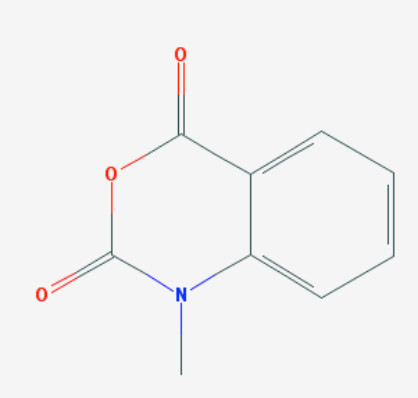
\includegraphics[scale=0.5]{lectures/160527/pix/NMIA.jpg} \\
(Quelle: $https://pubchem.ncbi.nlm.nih.gov/compound/N-Methylisatoic_anhydride$) \\

\item reverse Transkription: Die RNA wird mit DNA-Molekülen trankribiert.I m Anschluss werden die gewonnenen DNA-Fragmente sequenziert und als Library gespeichert
\item Da es auch zu zufälligen Abbruch bei der reversen Transkription kommen kann, wird ebenfalls eine negativ-Library erzeugt
\item Alignment der Reads an Transkriptom der RNA ($X_ij$, wobei i = Basenposition, j = Library)

\item Maximum-Likelihood-Model:

\begin{itemize}
\item $r_i = \dfrac{r_{i+}}{r_{i-}}$ $\rightarrow$ Datengrundlage
\item negativ-Library $\rightarrow$ Abbruchrate
\item simulierte Daten $m_i$ $\rightarrow$ Berechnung der positionsweisen Shape-Reaktivität 
\end{itemize}

\item[$\rightarrow$] Ermittlung der pseudo-Free-Energy

\begin{equation}
\Delta G_{Shape_i} = m * ln(\gamma_i * 1,0) + b
\end{equation}

\end{itemize}

m ... Anstieg des Bestrafungswertes \\
1,0 ... Pseudocount
b ... negativer Bonus der freien Energie für gepaarte Basen

\begin{equation}
M_{ij} = min
\begin{cases} 
M(i+1,j \\
min (M(i+1,k-1)*M(k+1,j)*e^{-\dfrac{E^{'}_{ij}}{kT}})
\end{cases}
\end{equation}

wobei:
\begin{equation}
E^{'}_{ij} = E_{ij} + \Delta G_{Shape_i} + \Delta G_{Shape_j}
\end{equation}

$E_{ij}$ ... Standard Energiemodell

\subsubsection{objective function approach}
\textbf{Hard constraints:} \\
$\rightarrow$ 3 Aussagen möglich: | = gepaart; . = ungepaart; X = unbekannt \\
\textbf{Soft constraints:} \\ 
$\rightarrow$ Wahrscheinlichkeit ob Base an Position Y gepaart ist oder nicht 

$\rightarrow$ Minimiere den Fehler F($\vec{E}$) \\
\begin{equation}
\vec{E} = \sum_{\mu} \dfrac{\varepsilon_{\mu}^{2}}{\tau^2} + \sum_{i = 0}^{n} \dfrac{1}{\sigma^2}(p_i(\vec{\varepsilon}) -q_i)^2
\end{equation} 

$\mu$ ... Strukturelemente
$\varepsilon_{\mu}$ ... Betrag der Stör-Energie eines Strukturelements\\
$\tau^2$ ... Varianz des Standardenergiemodells \\
$\sigma^2$ ... Varianz der Probingdaten \\
$p_i(\vec{\varepsilon})$ ... Wahrscheinlichkeit, dass i ungepaart ist unter Bedingung des Standardenergiemodells und der Störenergie

\subsubsection{Hydroxyl-Radikal Probing}
Hydroxyl-Radikale führen zum Bruch der RNA-Sequenz,wenn keine 3-D Interaktion stattfindet und keine Bindung an ein Protein vorliegt.\\
Nachteil: Sie sind nur kurzlebig in Lösung und müssen hergestellt werden

\subsubsection{DMS}
Di-Methylsulfat bindet an $CH_3$ von ungebundenen A bzw. C oder an eines der beiden, wenn sie das letzte Basenpaar einer Helix bilden oder wenn sie direkt neben einem GU-Basenpaar liegen. \\
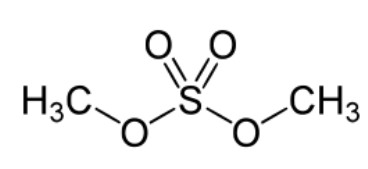
\includegraphics[scale=0.3]{lectures/160527/pix/Dimethylsulfat.jpg} \\

\subsubsection{CMCT}
(1-Cyclohexyl-(2-Morpholinoethyl)Carbodiimid Metho-p-Toluensulfonat) modifiziert vorwiegend ungepaartes Uridin und teilweise ungepaartes Guanin. \\
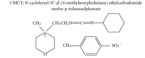
\includegraphics[scale=1]{lectures/160527/pix/CMCT.jpg} \\

\subsubsection{Kethoxal}
Kethoxal modifiziert ungepaartes Guanin \\
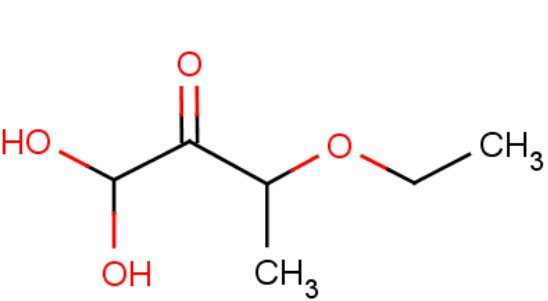
\includegraphics[scale=0.3]{lectures/160527/pix/Kethoxal.jpg}

\subsection{Nucleotide analoge interference mapping (NAIM)}
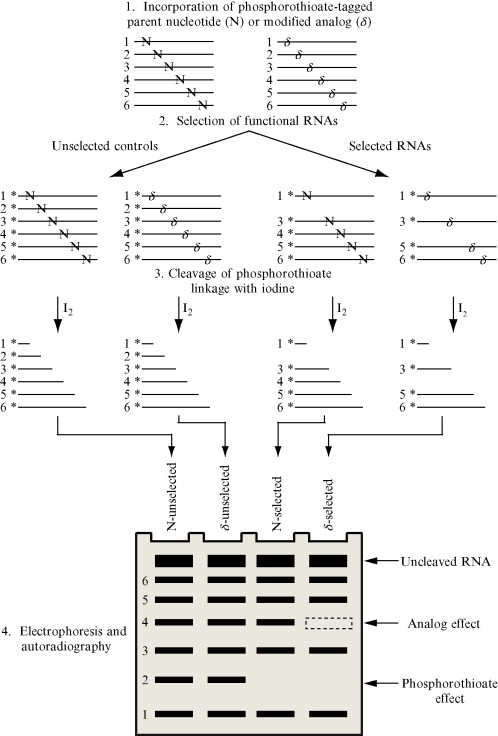
\includegraphics[scale=0.7]{lectures/160527/pix/NAIM.jpg} \\
(Quelle: http://www.sciencedirect.com/science/article/pii/S0076687909680010) \\
 
NAIM ist eine Erweiterung des Interferenz-Mappings mit Triphosphorsäure-Substitution
Untersucht, welche Basen funktional sind. Vorgehensweise:
\begin{itemize}
\item Nukleotide sind prinzipiell ohne funktionelle Gruppe
\item Nukleotide werden in vitro zufällig durch getaggede Analogika und getaggede normale Nukleotide während Transkription markiert
\item Annahme: Jedes Transkript hat nur ein getaggedes Nukleotid/Analogon
\item Auswahl der aktiven funktionalen RNAs und Erzeugung einer inaktiven Kontrollgruppe
\item Cleavage (Beschneiden) hinter der getaggeden Struktur durch Iod
\item Gelelektrophoresebild $\rightarrow$ gibt Aussage darüber welche durch Selektion sichtbar werden und welche durch Nukleotid-Einbau sichtbar sind
\end{itemize}

\newpage

\section{RNA structure probing}
\textbf{Bestimmung von:}
\begin{itemize}
\item Basenpaarung
\item Sekundärstruktur und Tertiärstruktur
\end{itemize}

\subsection{Inline-Probing}
inline-nucleophilic-attack: Wie in der Abbildung zu sehen kommt es zu strukturellen Änderungen der chemischen Konformation des RNA-Strangs an der Phosphatgruppe. Grund hierfür ist die Instabilität der Einzelsträngigen RNA, die bei Bindung eines Liganden an das Molekül zum Bruch ("Cleavage") führt oder eine rein zufällige Konformationsänderung des RNA-Moleküls. \\
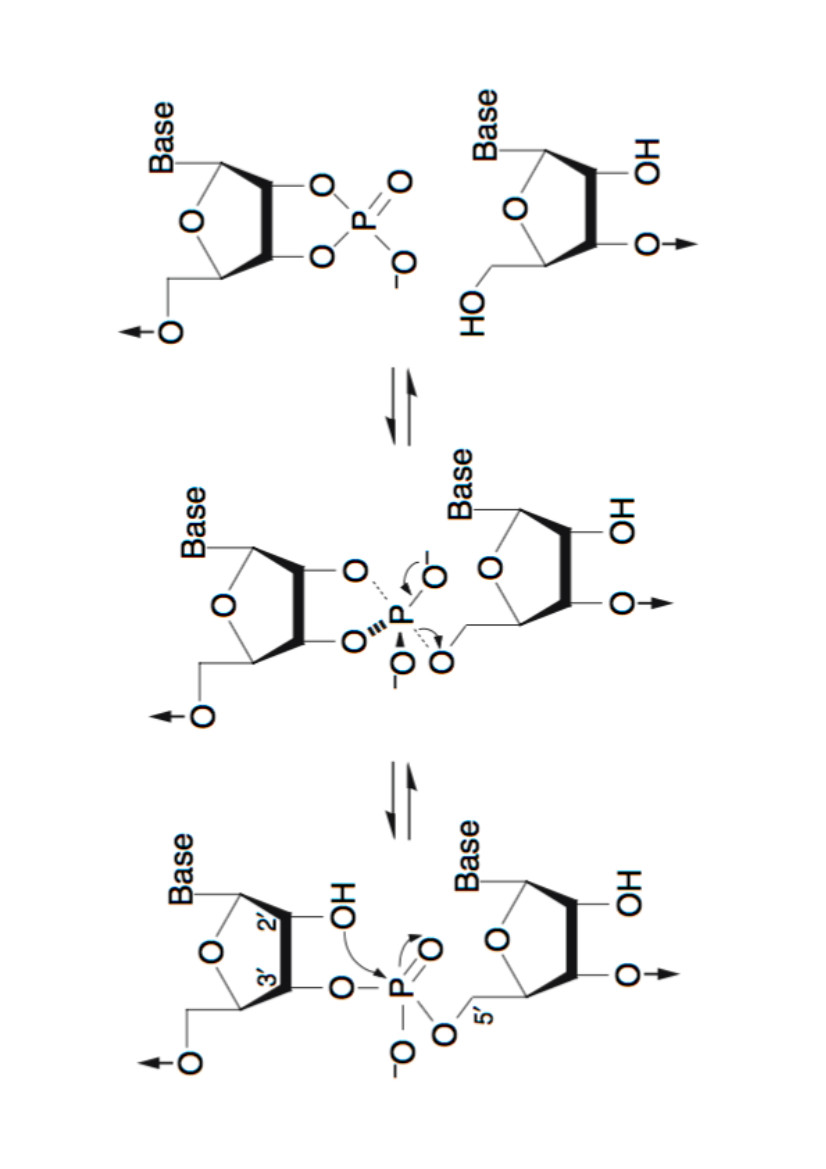
\includegraphics[scale=0.25,angle=270]{lectures/160527/pix/inline.jpg}

\textbf{Vorgehen:}
\begin{itemize}
\item Erstellen von zwei Proben des zu untersuchenden RNA-Moleküls
\item In einer Probe gewählten Ligand hinzugeben
\item beide Proben werden lange inkubiert $\rightarrow$ nucleophilic attack
\item Gelbild mittels Gelelektrophorese herstellen und Längen der RNA-Fragmente beider Proben vergleichend betrachten
\item gleiche Strukturen werden als Hintergrundrauschen (ligandenunabhängige) Cleavages betrachtet
\end{itemize}

\subsection{Chemisches Probing}
RNA-modifizierende Chemikalien sind \textbf{struktursensitiv} [1] und \textbf{sequenzunabhängig} \\
\begin{itemize}
\item[1] Es werden Chemikalien genutzt die entweder gepaarte oder ungepaarte Basen modifizieren
\item[2] Mechanismus zur Detektion der Modifikation
\end{itemize}

\subsubsection{SHAPE-Seq}
(\textbf{S}elective 2'-\textbf{h}ydroxylacetylation \textbf{a}nalyzed by \textbf{p}rimer \textbf{e}xtention \textbf{seq}uencing)

\begin{itemize}
\item 2'-OH ist reaktiver wenn die zugehörige Base ungebunden ist
\item genutzte Chemikalie: N-methylisatoic anhybdride
\item unter Abgabe von Kohlenstoffdioxid ($CO_2$) bindet ein Sauerstoffmolekül des NMIA an 2'-OH der RNA \\
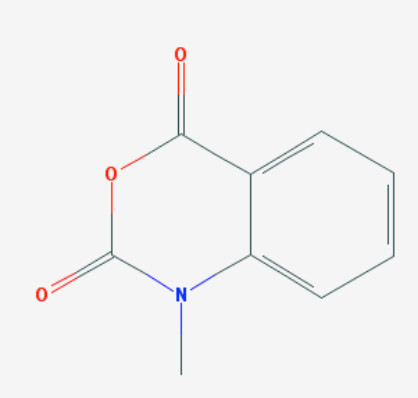
\includegraphics[scale=0.5]{lectures/160527/pix/NMIA.jpg} \\
(Quelle: $https://pubchem.ncbi.nlm.nih.gov/compound/N-Methylisatoic_anhydride$) \\

\item reverse Transkription: Die RNA wird mit DNA-Molekülen trankribiert.I m Anschluss werden die gewonnenen DNA-Fragmente sequenziert und als Library gespeichert
\item Da es auch zu zufälligen Abbruch bei der reversen Transkription kommen kann, wird ebenfalls eine negativ-Library erzeugt
\item Alignment der Reads an Transkriptom der RNA ($X_ij$, wobei i = Basenposition, j = Library)

\item Maximum-Likelihood-Model:

\begin{itemize}
\item $r_i = \dfrac{r_{i+}}{r_{i-}}$ $\rightarrow$ Datengrundlage
\item negativ-Library $\rightarrow$ Abbruchrate
\item simulierte Daten $m_i$ $\rightarrow$ Berechnung der positionsweisen Shape-Reaktivität 
\end{itemize}

\item[$\rightarrow$] Ermittlung der pseudo-Free-Energy

\begin{equation}
\Delta G_{Shape_i} = m * ln(\gamma_i * 1,0) + b
\end{equation}

\end{itemize}

m ... Anstieg des Bestrafungswertes \\
1,0 ... Pseudocount
b ... negativer Bonus der freien Energie für gepaarte Basen

\begin{equation}
M_{ij} = min
\begin{cases} 
M(i+1,j \\
min (M(i+1,k-1)*M(k+1,j)*e^{-\dfrac{E^{'}_{ij}}{kT}})
\end{cases}
\end{equation}

wobei:
\begin{equation}
E^{'}_{ij} = E_{ij} + \Delta G_{Shape_i} + \Delta G_{Shape_j}
\end{equation}

$E_{ij}$ ... Standard Energiemodell

\subsubsection{objective function approach}
\textbf{Hard constraints:} \\
$\rightarrow$ 3 Aussagen möglich: | = gepaart; . = ungepaart; X = unbekannt \\
\textbf{Soft constraints:} \\ 
$\rightarrow$ Wahrscheinlichkeit ob Base an Position Y gepaart ist oder nicht 

$\rightarrow$ Minimiere den Fehler F($\vec{E}$) \\
\begin{equation}
\vec{E} = \sum_{\mu} \dfrac{\varepsilon_{\mu}^{2}}{\tau^2} + \sum_{i = 0}^{n} \dfrac{1}{\sigma^2}(p_i(\vec{\varepsilon}) -q_i)^2
\end{equation} 

$\mu$ ... Strukturelemente
$\varepsilon_{\mu}$ ... Betrag der Stör-Energie eines Strukturelements\\
$\tau^2$ ... Varianz des Standardenergiemodells \\
$\sigma^2$ ... Varianz der Probingdaten \\
$p_i(\vec{\varepsilon})$ ... Wahrscheinlichkeit, dass i ungepaart ist unter Bedingung des Standardenergiemodells und der Störenergie

\subsubsection{Hydroxyl-Radikal Probing}
Hydroxyl-Radikale führen zum Bruch der RNA-Sequenz,wenn keine 3-D Interaktion stattfindet und keine Bindung an ein Protein vorliegt.\\
Nachteil: Sie sind nur kurzlebig in Lösung und müssen hergestellt werden

\subsubsection{DMS}
Di-Methylsulfat bindet an $CH_3$ von ungebundenen A bzw. C oder an eines der beiden, wenn sie das letzte Basenpaar einer Helix bilden oder wenn sie direkt neben einem GU-Basenpaar liegen. \\
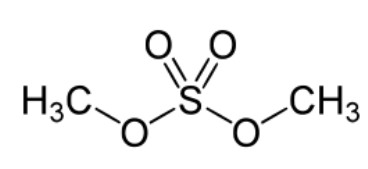
\includegraphics[scale=0.3]{lectures/160527/pix/Dimethylsulfat.jpg} \\

\subsubsection{CMCT}
(1-Cyclohexyl-(2-Morpholinoethyl)Carbodiimid Metho-p-Toluensulfonat) modifiziert vorwiegend ungepaartes Uridin und teilweise ungepaartes Guanin. \\
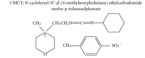
\includegraphics[scale=1]{lectures/160527/pix/CMCT.jpg} \\

\subsubsection{Kethoxal}
Kethoxal modifiziert ungepaartes Guanin \\
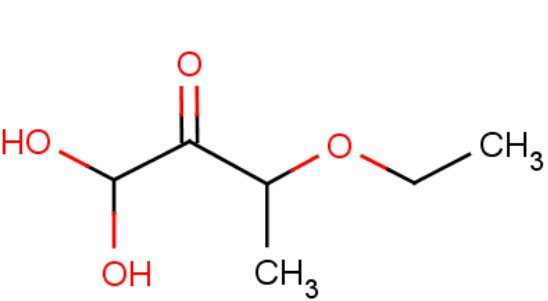
\includegraphics[scale=0.3]{lectures/160527/pix/Kethoxal.jpg}

\subsection{Nucleotide analoge interference mapping (NAIM)}
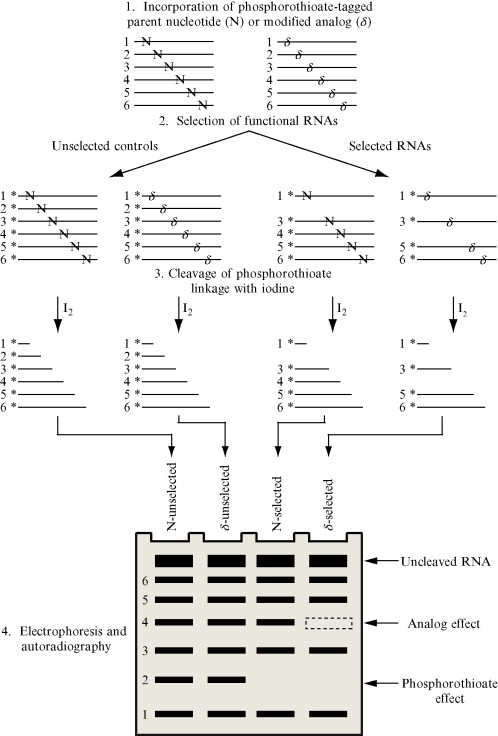
\includegraphics[scale=0.7]{lectures/160527/pix/NAIM.jpg} \\
(Quelle: http://www.sciencedirect.com/science/article/pii/S0076687909680010) \\
 
NAIM ist eine Erweiterung des Interferenz-Mappings mit Triphosphorsäure-Substitution
Untersucht, welche Basen funktional sind. Vorgehensweise:
\begin{itemize}
\item Nukleotide sind prinzipiell ohne funktionelle Gruppe
\item Nukleotide werden in vitro zufällig durch getaggede Analogika und getaggede normale Nukleotide während Transkription markiert
\item Annahme: Jedes Transkript hat nur ein getaggedes Nukleotid/Analogon
\item Auswahl der aktiven funktionalen RNAs und Erzeugung einer inaktiven Kontrollgruppe
\item Cleavage (Beschneiden) hinter der getaggeden Struktur durch Iod
\item Gelelektrophoresebild $\rightarrow$ gibt Aussage darüber welche durch Selektion sichtbar werden und welche durch Nukleotid-Einbau sichtbar sind
\end{itemize}

\newpage

\section{RNA structure probing}
\textbf{Bestimmung von:}
\begin{itemize}
\item Basenpaarung
\item Sekundärstruktur und Tertiärstruktur
\end{itemize}

\subsection{Inline-Probing}
inline-nucleophilic-attack: Wie in der Abbildung zu sehen kommt es zu strukturellen Änderungen der chemischen Konformation des RNA-Strangs an der Phosphatgruppe. Grund hierfür ist die Instabilität der Einzelsträngigen RNA, die bei Bindung eines Liganden an das Molekül zum Bruch ("Cleavage") führt oder eine rein zufällige Konformationsänderung des RNA-Moleküls. \\
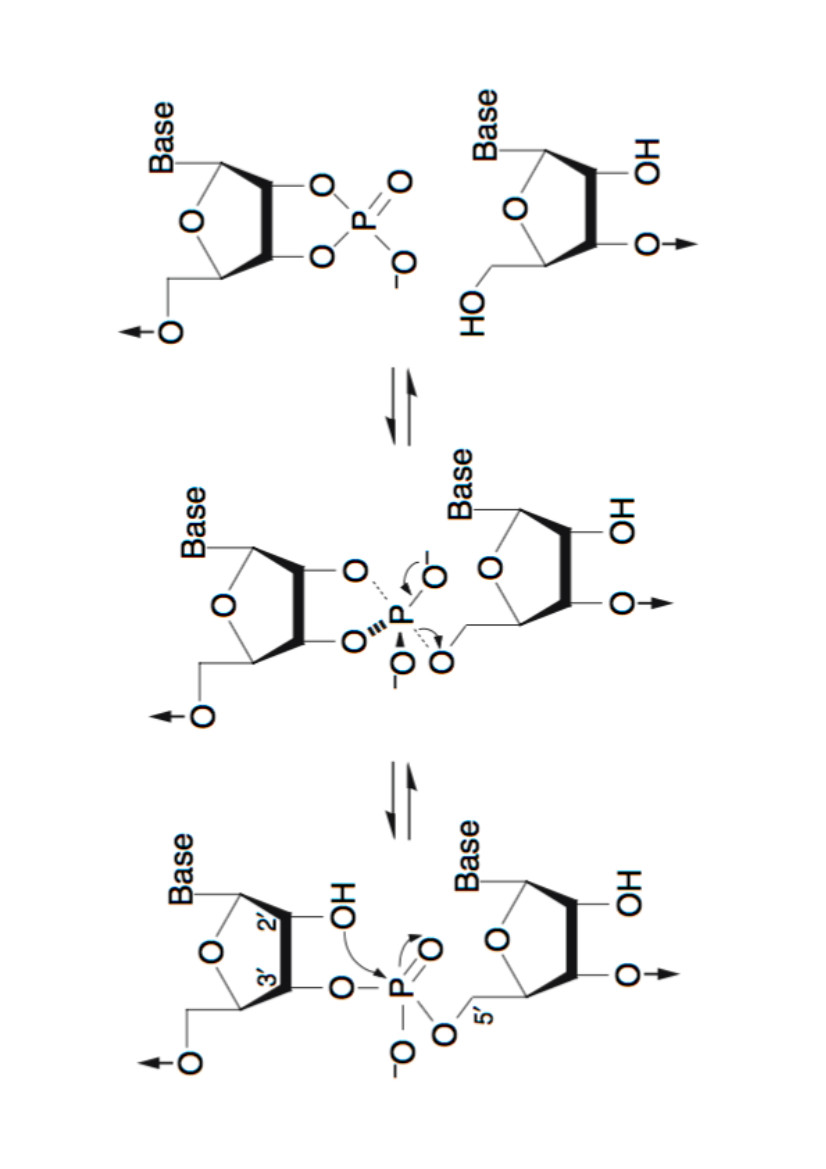
\includegraphics[scale=0.25,angle=270]{lectures/160527/pix/inline.jpg}

\textbf{Vorgehen:}
\begin{itemize}
\item Erstellen von zwei Proben des zu untersuchenden RNA-Moleküls
\item In einer Probe gewählten Ligand hinzugeben
\item beide Proben werden lange inkubiert $\rightarrow$ nucleophilic attack
\item Gelbild mittels Gelelektrophorese herstellen und Längen der RNA-Fragmente beider Proben vergleichend betrachten
\item gleiche Strukturen werden als Hintergrundrauschen (ligandenunabhängige) Cleavages betrachtet
\end{itemize}

\subsection{Chemisches Probing}
RNA-modifizierende Chemikalien sind \textbf{struktursensitiv} [1] und \textbf{sequenzunabhängig} \\
\begin{itemize}
\item[1] Es werden Chemikalien genutzt die entweder gepaarte oder ungepaarte Basen modifizieren
\item[2] Mechanismus zur Detektion der Modifikation
\end{itemize}

\subsubsection{SHAPE-Seq}
(\textbf{S}elective 2'-\textbf{h}ydroxylacetylation \textbf{a}nalyzed by \textbf{p}rimer \textbf{e}xtention \textbf{seq}uencing)

\begin{itemize}
\item 2'-OH ist reaktiver wenn die zugehörige Base ungebunden ist
\item genutzte Chemikalie: N-methylisatoic anhybdride
\item unter Abgabe von Kohlenstoffdioxid ($CO_2$) bindet ein Sauerstoffmolekül des NMIA an 2'-OH der RNA \\
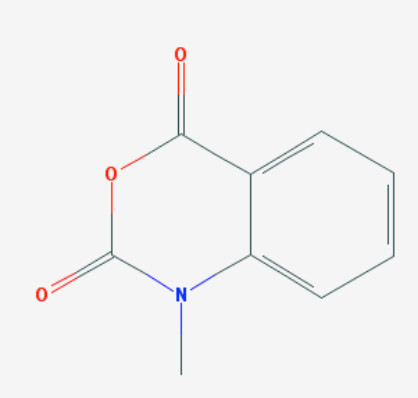
\includegraphics[scale=0.5]{lectures/160527/pix/NMIA.jpg} \\
(Quelle: $https://pubchem.ncbi.nlm.nih.gov/compound/N-Methylisatoic_anhydride$) \\

\item reverse Transkription: Die RNA wird mit DNA-Molekülen trankribiert.I m Anschluss werden die gewonnenen DNA-Fragmente sequenziert und als Library gespeichert
\item Da es auch zu zufälligen Abbruch bei der reversen Transkription kommen kann, wird ebenfalls eine negativ-Library erzeugt
\item Alignment der Reads an Transkriptom der RNA ($X_ij$, wobei i = Basenposition, j = Library)

\item Maximum-Likelihood-Model:

\begin{itemize}
\item $r_i = \dfrac{r_{i+}}{r_{i-}}$ $\rightarrow$ Datengrundlage
\item negativ-Library $\rightarrow$ Abbruchrate
\item simulierte Daten $m_i$ $\rightarrow$ Berechnung der positionsweisen Shape-Reaktivität 
\end{itemize}

\item[$\rightarrow$] Ermittlung der pseudo-Free-Energy

\begin{equation}
\Delta G_{Shape_i} = m * ln(\gamma_i * 1,0) + b
\end{equation}

\end{itemize}

m ... Anstieg des Bestrafungswertes \\
1,0 ... Pseudocount
b ... negativer Bonus der freien Energie für gepaarte Basen

\begin{equation}
M_{ij} = min
\begin{cases} 
M(i+1,j \\
min (M(i+1,k-1)*M(k+1,j)*e^{-\dfrac{E^{'}_{ij}}{kT}})
\end{cases}
\end{equation}

wobei:
\begin{equation}
E^{'}_{ij} = E_{ij} + \Delta G_{Shape_i} + \Delta G_{Shape_j}
\end{equation}

$E_{ij}$ ... Standard Energiemodell

\subsubsection{objective function approach}
\textbf{Hard constraints:} \\
$\rightarrow$ 3 Aussagen möglich: | = gepaart; . = ungepaart; X = unbekannt \\
\textbf{Soft constraints:} \\ 
$\rightarrow$ Wahrscheinlichkeit ob Base an Position Y gepaart ist oder nicht 

$\rightarrow$ Minimiere den Fehler F($\vec{E}$) \\
\begin{equation}
\vec{E} = \sum_{\mu} \dfrac{\varepsilon_{\mu}^{2}}{\tau^2} + \sum_{i = 0}^{n} \dfrac{1}{\sigma^2}(p_i(\vec{\varepsilon}) -q_i)^2
\end{equation} 

$\mu$ ... Strukturelemente
$\varepsilon_{\mu}$ ... Betrag der Stör-Energie eines Strukturelements\\
$\tau^2$ ... Varianz des Standardenergiemodells \\
$\sigma^2$ ... Varianz der Probingdaten \\
$p_i(\vec{\varepsilon})$ ... Wahrscheinlichkeit, dass i ungepaart ist unter Bedingung des Standardenergiemodells und der Störenergie

\subsubsection{Hydroxyl-Radikal Probing}
Hydroxyl-Radikale führen zum Bruch der RNA-Sequenz,wenn keine 3-D Interaktion stattfindet und keine Bindung an ein Protein vorliegt.\\
Nachteil: Sie sind nur kurzlebig in Lösung und müssen hergestellt werden

\subsubsection{DMS}
Di-Methylsulfat bindet an $CH_3$ von ungebundenen A bzw. C oder an eines der beiden, wenn sie das letzte Basenpaar einer Helix bilden oder wenn sie direkt neben einem GU-Basenpaar liegen. \\
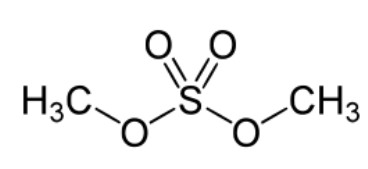
\includegraphics[scale=0.3]{lectures/160527/pix/Dimethylsulfat.jpg} \\

\subsubsection{CMCT}
(1-Cyclohexyl-(2-Morpholinoethyl)Carbodiimid Metho-p-Toluensulfonat) modifiziert vorwiegend ungepaartes Uridin und teilweise ungepaartes Guanin. \\
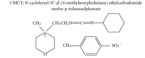
\includegraphics[scale=1]{lectures/160527/pix/CMCT.jpg} \\

\subsubsection{Kethoxal}
Kethoxal modifiziert ungepaartes Guanin \\
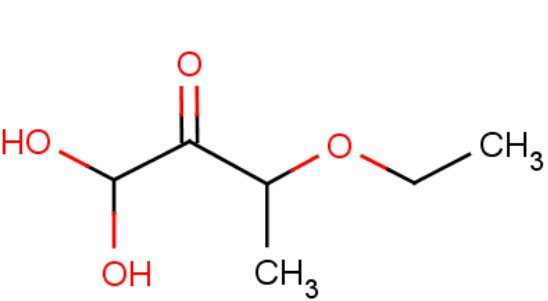
\includegraphics[scale=0.3]{lectures/160527/pix/Kethoxal.jpg}

\subsection{Nucleotide analoge interference mapping (NAIM)}
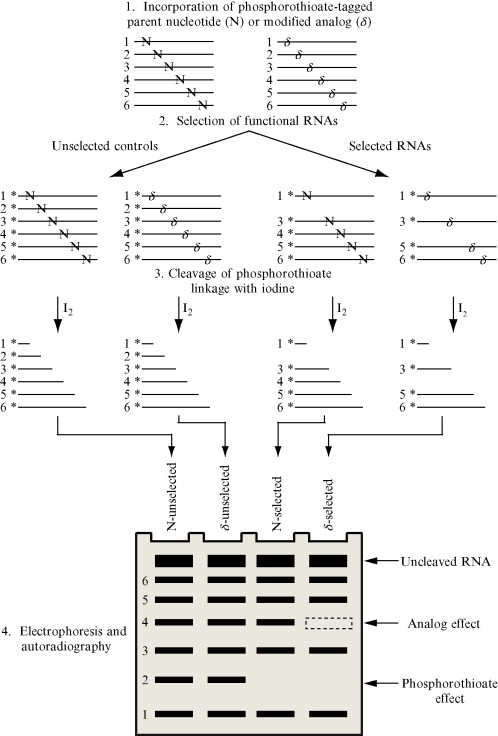
\includegraphics[scale=0.7]{lectures/160527/pix/NAIM.jpg} \\
(Quelle: http://www.sciencedirect.com/science/article/pii/S0076687909680010) \\
 
NAIM ist eine Erweiterung des Interferenz-Mappings mit Triphosphorsäure-Substitution
Untersucht, welche Basen funktional sind. Vorgehensweise:
\begin{itemize}
\item Nukleotide sind prinzipiell ohne funktionelle Gruppe
\item Nukleotide werden in vitro zufällig durch getaggede Analogika und getaggede normale Nukleotide während Transkription markiert
\item Annahme: Jedes Transkript hat nur ein getaggedes Nukleotid/Analogon
\item Auswahl der aktiven funktionalen RNAs und Erzeugung einer inaktiven Kontrollgruppe
\item Cleavage (Beschneiden) hinter der getaggeden Struktur durch Iod
\item Gelelektrophoresebild $\rightarrow$ gibt Aussage darüber welche durch Selektion sichtbar werden und welche durch Nukleotid-Einbau sichtbar sind
\end{itemize}

\newpage

\section{RNA structure probing}
\textbf{Bestimmung von:}
\begin{itemize}
\item Basenpaarung
\item Sekundärstruktur und Tertiärstruktur
\end{itemize}

\subsection{Inline-Probing}
inline-nucleophilic-attack: Wie in der Abbildung zu sehen kommt es zu strukturellen Änderungen der chemischen Konformation des RNA-Strangs an der Phosphatgruppe. Grund hierfür ist die Instabilität der Einzelsträngigen RNA, die bei Bindung eines Liganden an das Molekül zum Bruch ("Cleavage") führt oder eine rein zufällige Konformationsänderung des RNA-Moleküls. \\
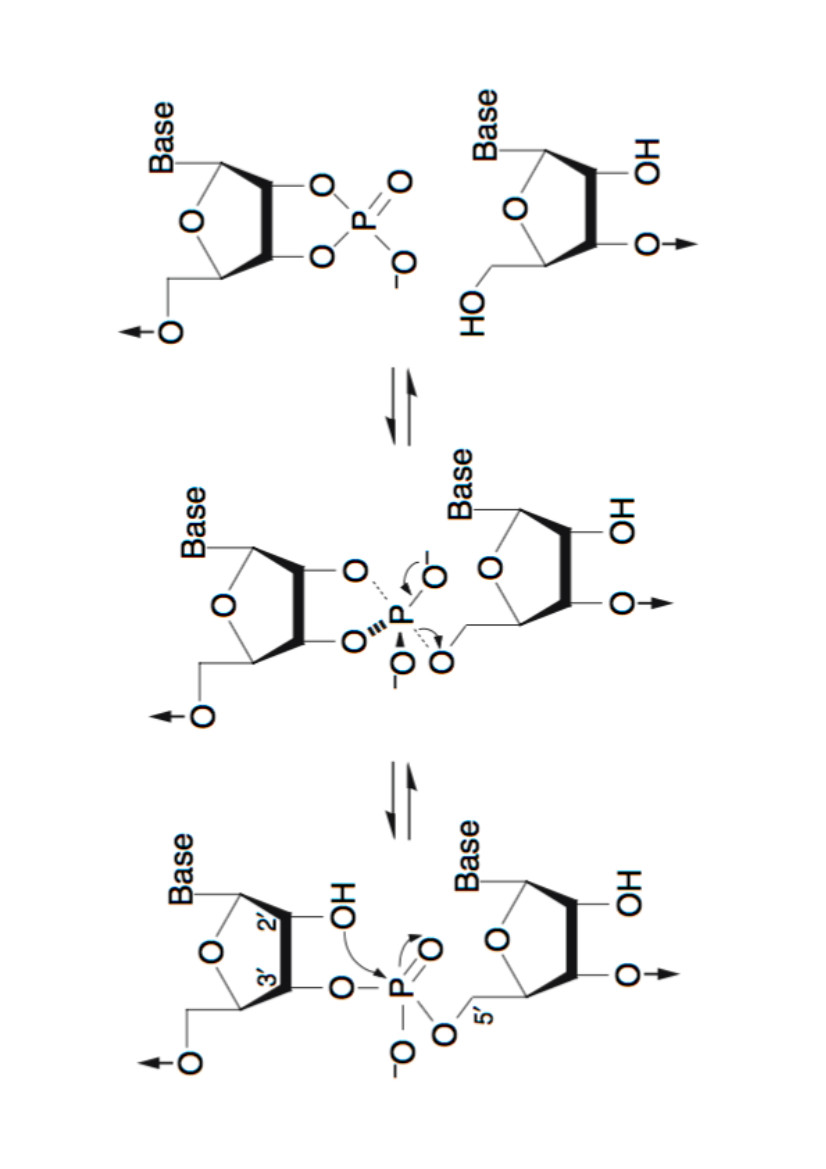
\includegraphics[scale=0.25,angle=270]{lectures/160527/pix/inline.jpg}

\textbf{Vorgehen:}
\begin{itemize}
\item Erstellen von zwei Proben des zu untersuchenden RNA-Moleküls
\item In einer Probe gewählten Ligand hinzugeben
\item beide Proben werden lange inkubiert $\rightarrow$ nucleophilic attack
\item Gelbild mittels Gelelektrophorese herstellen und Längen der RNA-Fragmente beider Proben vergleichend betrachten
\item gleiche Strukturen werden als Hintergrundrauschen (ligandenunabhängige) Cleavages betrachtet
\end{itemize}

\subsection{Chemisches Probing}
RNA-modifizierende Chemikalien sind \textbf{struktursensitiv} [1] und \textbf{sequenzunabhängig} \\
\begin{itemize}
\item[1] Es werden Chemikalien genutzt die entweder gepaarte oder ungepaarte Basen modifizieren
\item[2] Mechanismus zur Detektion der Modifikation
\end{itemize}

\subsubsection{SHAPE-Seq}
(\textbf{S}elective 2'-\textbf{h}ydroxylacetylation \textbf{a}nalyzed by \textbf{p}rimer \textbf{e}xtention \textbf{seq}uencing)

\begin{itemize}
\item 2'-OH ist reaktiver wenn die zugehörige Base ungebunden ist
\item genutzte Chemikalie: N-methylisatoic anhybdride
\item unter Abgabe von Kohlenstoffdioxid ($CO_2$) bindet ein Sauerstoffmolekül des NMIA an 2'-OH der RNA \\
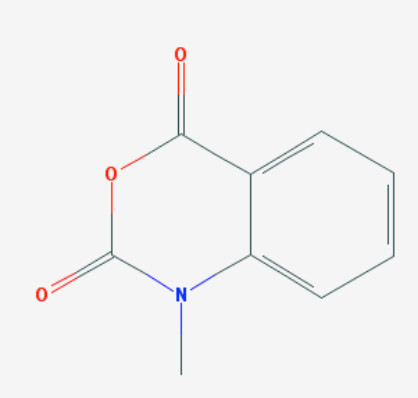
\includegraphics[scale=0.5]{lectures/160527/pix/NMIA.jpg} \\
(Quelle: $https://pubchem.ncbi.nlm.nih.gov/compound/N-Methylisatoic_anhydride$) \\

\item reverse Transkription: Die RNA wird mit DNA-Molekülen trankribiert.I m Anschluss werden die gewonnenen DNA-Fragmente sequenziert und als Library gespeichert
\item Da es auch zu zufälligen Abbruch bei der reversen Transkription kommen kann, wird ebenfalls eine negativ-Library erzeugt
\item Alignment der Reads an Transkriptom der RNA ($X_ij$, wobei i = Basenposition, j = Library)

\item Maximum-Likelihood-Model:

\begin{itemize}
\item $r_i = \dfrac{r_{i+}}{r_{i-}}$ $\rightarrow$ Datengrundlage
\item negativ-Library $\rightarrow$ Abbruchrate
\item simulierte Daten $m_i$ $\rightarrow$ Berechnung der positionsweisen Shape-Reaktivität 
\end{itemize}

\item[$\rightarrow$] Ermittlung der pseudo-Free-Energy

\begin{equation}
\Delta G_{Shape_i} = m * ln(\gamma_i * 1,0) + b
\end{equation}

\end{itemize}

m ... Anstieg des Bestrafungswertes \\
1,0 ... Pseudocount
b ... negativer Bonus der freien Energie für gepaarte Basen

\begin{equation}
M_{ij} = min
\begin{cases} 
M(i+1,j \\
min (M(i+1,k-1)*M(k+1,j)*e^{-\dfrac{E^{'}_{ij}}{kT}})
\end{cases}
\end{equation}

wobei:
\begin{equation}
E^{'}_{ij} = E_{ij} + \Delta G_{Shape_i} + \Delta G_{Shape_j}
\end{equation}

$E_{ij}$ ... Standard Energiemodell

\subsubsection{objective function approach}
\textbf{Hard constraints:} \\
$\rightarrow$ 3 Aussagen möglich: | = gepaart; . = ungepaart; X = unbekannt \\
\textbf{Soft constraints:} \\ 
$\rightarrow$ Wahrscheinlichkeit ob Base an Position Y gepaart ist oder nicht 

$\rightarrow$ Minimiere den Fehler F($\vec{E}$) \\
\begin{equation}
\vec{E} = \sum_{\mu} \dfrac{\varepsilon_{\mu}^{2}}{\tau^2} + \sum_{i = 0}^{n} \dfrac{1}{\sigma^2}(p_i(\vec{\varepsilon}) -q_i)^2
\end{equation} 

$\mu$ ... Strukturelemente
$\varepsilon_{\mu}$ ... Betrag der Stör-Energie eines Strukturelements\\
$\tau^2$ ... Varianz des Standardenergiemodells \\
$\sigma^2$ ... Varianz der Probingdaten \\
$p_i(\vec{\varepsilon})$ ... Wahrscheinlichkeit, dass i ungepaart ist unter Bedingung des Standardenergiemodells und der Störenergie

\subsubsection{Hydroxyl-Radikal Probing}
Hydroxyl-Radikale führen zum Bruch der RNA-Sequenz,wenn keine 3-D Interaktion stattfindet und keine Bindung an ein Protein vorliegt.\\
Nachteil: Sie sind nur kurzlebig in Lösung und müssen hergestellt werden

\subsubsection{DMS}
Di-Methylsulfat bindet an $CH_3$ von ungebundenen A bzw. C oder an eines der beiden, wenn sie das letzte Basenpaar einer Helix bilden oder wenn sie direkt neben einem GU-Basenpaar liegen. \\
\includegraphics[scale=0.3]{lectures/160527/pix/Dimethylsulfat.jpg} \\

\subsubsection{CMCT}
(1-Cyclohexyl-(2-Morpholinoethyl)Carbodiimid Metho-p-Toluensulfonat) modifiziert vorwiegend ungepaartes Uridin und teilweise ungepaartes Guanin. \\
\includegraphics[scale=1]{lectures/160527/pix/CMCT.jpg} \\

\subsubsection{Kethoxal}
Kethoxal modifiziert ungepaartes Guanin \\
\includegraphics[scale=0.3]{lectures/160527/pix/Kethoxal.jpg}

\subsection{Nucleotide analoge interference mapping (NAIM)}
\includegraphics[scale=0.7]{lectures/160527/pix/NAIM.jpg} \\
(Quelle: http://www.sciencedirect.com/science/article/pii/S0076687909680010) \\
 
NAIM ist eine Erweiterung des Interferenz-Mappings mit Triphosphorsäure-Substitution
Untersucht, welche Basen funktional sind. Vorgehensweise:
\begin{itemize}
\item Nukleotide sind prinzipiell ohne funktionelle Gruppe
\item Nukleotide werden in vitro zufällig durch getaggede Analogika und getaggede normale Nukleotide während Transkription markiert
\item Annahme: Jedes Transkript hat nur ein getaggedes Nukleotid/Analogon
\item Auswahl der aktiven funktionalen RNAs und Erzeugung einer inaktiven Kontrollgruppe
\item Cleavage (Beschneiden) hinter der getaggeden Struktur durch Iod
\item Gelelektrophoresebild $\rightarrow$ gibt Aussage darüber welche durch Selektion sichtbar werden und welche durch Nukleotid-Einbau sichtbar sind
\end{itemize}

\newpage

\section{RNA structure probing}
\textbf{Bestimmung von:}
\begin{itemize}
\item Basenpaarung
\item Sekundärstruktur und Tertiärstruktur
\end{itemize}

\subsection{Inline-Probing}
inline-nucleophilic-attack: Wie in der Abbildung zu sehen kommt es zu strukturellen Änderungen der chemischen Konformation des RNA-Strangs an der Phosphatgruppe. Grund hierfür ist die Instabilität der Einzelsträngigen RNA, die bei Bindung eines Liganden an das Molekül zum Bruch ("Cleavage") führt oder eine rein zufällige Konformationsänderung des RNA-Moleküls. \\
\includegraphics[scale=0.25,angle=270]{lectures/160527/pix/inline.jpg}

\textbf{Vorgehen:}
\begin{itemize}
\item Erstellen von zwei Proben des zu untersuchenden RNA-Moleküls
\item In einer Probe gewählten Ligand hinzugeben
\item beide Proben werden lange inkubiert $\rightarrow$ nucleophilic attack
\item Gelbild mittels Gelelektrophorese herstellen und Längen der RNA-Fragmente beider Proben vergleichend betrachten
\item gleiche Strukturen werden als Hintergrundrauschen (ligandenunabhängige) Cleavages betrachtet
\end{itemize}

\subsection{Chemisches Probing}
RNA-modifizierende Chemikalien sind \textbf{struktursensitiv} [1] und \textbf{sequenzunabhängig} \\
\begin{itemize}
\item[1] Es werden Chemikalien genutzt die entweder gepaarte oder ungepaarte Basen modifizieren
\item[2] Mechanismus zur Detektion der Modifikation
\end{itemize}

\subsubsection{SHAPE-Seq}
(\textbf{S}elective 2'-\textbf{h}ydroxylacetylation \textbf{a}nalyzed by \textbf{p}rimer \textbf{e}xtention \textbf{seq}uencing)

\begin{itemize}
\item 2'-OH ist reaktiver wenn die zugehörige Base ungebunden ist
\item genutzte Chemikalie: N-methylisatoic anhybdride
\item unter Abgabe von Kohlenstoffdioxid ($CO_2$) bindet ein Sauerstoffmolekül des NMIA an 2'-OH der RNA \\
\includegraphics[scale=0.5]{lectures/160527/pix/NMIA.jpg} \\
(Quelle: $https://pubchem.ncbi.nlm.nih.gov/compound/N-Methylisatoic_anhydride$) \\

\item reverse Transkription: Die RNA wird mit DNA-Molekülen trankribiert.I m Anschluss werden die gewonnenen DNA-Fragmente sequenziert und als Library gespeichert
\item Da es auch zu zufälligen Abbruch bei der reversen Transkription kommen kann, wird ebenfalls eine negativ-Library erzeugt
\item Alignment der Reads an Transkriptom der RNA ($X_ij$, wobei i = Basenposition, j = Library)

\item Maximum-Likelihood-Model:

\begin{itemize}
\item $r_i = \dfrac{r_{i+}}{r_{i-}}$ $\rightarrow$ Datengrundlage
\item negativ-Library $\rightarrow$ Abbruchrate
\item simulierte Daten $m_i$ $\rightarrow$ Berechnung der positionsweisen Shape-Reaktivität 
\end{itemize}

\item[$\rightarrow$] Ermittlung der pseudo-Free-Energy

\begin{equation}
\Delta G_{Shape_i} = m * ln(\gamma_i * 1,0) + b
\end{equation}

\end{itemize}

m ... Anstieg des Bestrafungswertes \\
1,0 ... Pseudocount
b ... negativer Bonus der freien Energie für gepaarte Basen

\begin{equation}
M_{ij} = min
\begin{cases} 
M(i+1,j \\
min (M(i+1,k-1)*M(k+1,j)*e^{-\dfrac{E^{'}_{ij}}{kT}})
\end{cases}
\end{equation}

wobei:
\begin{equation}
E^{'}_{ij} = E_{ij} + \Delta G_{Shape_i} + \Delta G_{Shape_j}
\end{equation}

$E_{ij}$ ... Standard Energiemodell

\subsubsection{objective function approach}
\textbf{Hard constraints:} \\
$\rightarrow$ 3 Aussagen möglich: | = gepaart; . = ungepaart; X = unbekannt \\
\textbf{Soft constraints:} \\ 
$\rightarrow$ Wahrscheinlichkeit ob Base an Position Y gepaart ist oder nicht 

$\rightarrow$ Minimiere den Fehler F($\vec{E}$) \\
\begin{equation}
\vec{E} = \sum_{\mu} \dfrac{\varepsilon_{\mu}^{2}}{\tau^2} + \sum_{i = 0}^{n} \dfrac{1}{\sigma^2}(p_i(\vec{\varepsilon}) -q_i)^2
\end{equation} 

$\mu$ ... Strukturelemente
$\varepsilon_{\mu}$ ... Betrag der Stör-Energie eines Strukturelements\\
$\tau^2$ ... Varianz des Standardenergiemodells \\
$\sigma^2$ ... Varianz der Probingdaten \\
$p_i(\vec{\varepsilon})$ ... Wahrscheinlichkeit, dass i ungepaart ist unter Bedingung des Standardenergiemodells und der Störenergie

\subsubsection{Hydroxyl-Radikal Probing}
Hydroxyl-Radikale führen zum Bruch der RNA-Sequenz,wenn keine 3-D Interaktion stattfindet und keine Bindung an ein Protein vorliegt.\\
Nachteil: Sie sind nur kurzlebig in Lösung und müssen hergestellt werden

\subsubsection{DMS}
Di-Methylsulfat bindet an $CH_3$ von ungebundenen A bzw. C oder an eines der beiden, wenn sie das letzte Basenpaar einer Helix bilden oder wenn sie direkt neben einem GU-Basenpaar liegen. \\
\includegraphics[scale=0.3]{lectures/160527/pix/Dimethylsulfat.jpg} \\

\subsubsection{CMCT}
(1-Cyclohexyl-(2-Morpholinoethyl)Carbodiimid Metho-p-Toluensulfonat) modifiziert vorwiegend ungepaartes Uridin und teilweise ungepaartes Guanin. \\
\includegraphics[scale=1]{lectures/160527/pix/CMCT.jpg} \\

\subsubsection{Kethoxal}
Kethoxal modifiziert ungepaartes Guanin \\
\includegraphics[scale=0.3]{lectures/160527/pix/Kethoxal.jpg}

\subsection{Nucleotide analoge interference mapping (NAIM)}
\includegraphics[scale=0.7]{lectures/160527/pix/NAIM.jpg} \\
(Quelle: http://www.sciencedirect.com/science/article/pii/S0076687909680010) \\
 
NAIM ist eine Erweiterung des Interferenz-Mappings mit Triphosphorsäure-Substitution
Untersucht, welche Basen funktional sind. Vorgehensweise:
\begin{itemize}
\item Nukleotide sind prinzipiell ohne funktionelle Gruppe
\item Nukleotide werden in vitro zufällig durch getaggede Analogika und getaggede normale Nukleotide während Transkription markiert
\item Annahme: Jedes Transkript hat nur ein getaggedes Nukleotid/Analogon
\item Auswahl der aktiven funktionalen RNAs und Erzeugung einer inaktiven Kontrollgruppe
\item Cleavage (Beschneiden) hinter der getaggeden Struktur durch Iod
\item Gelelektrophoresebild $\rightarrow$ gibt Aussage darüber welche durch Selektion sichtbar werden und welche durch Nukleotid-Einbau sichtbar sind
\end{itemize}

\newpage

\section{RNA structure probing}
\textbf{Bestimmung von:}
\begin{itemize}
\item Basenpaarung
\item Sekundärstruktur und Tertiärstruktur
\end{itemize}

\subsection{Inline-Probing}
inline-nucleophilic-attack: Wie in der Abbildung zu sehen kommt es zu strukturellen Änderungen der chemischen Konformation des RNA-Strangs an der Phosphatgruppe. Grund hierfür ist die Instabilität der Einzelsträngigen RNA, die bei Bindung eines Liganden an das Molekül zum Bruch ("Cleavage") führt oder eine rein zufällige Konformationsänderung des RNA-Moleküls. \\
\includegraphics[scale=0.25,angle=270]{lectures/160527/pix/inline.jpg}

\textbf{Vorgehen:}
\begin{itemize}
\item Erstellen von zwei Proben des zu untersuchenden RNA-Moleküls
\item In einer Probe gewählten Ligand hinzugeben
\item beide Proben werden lange inkubiert $\rightarrow$ nucleophilic attack
\item Gelbild mittels Gelelektrophorese herstellen und Längen der RNA-Fragmente beider Proben vergleichend betrachten
\item gleiche Strukturen werden als Hintergrundrauschen (ligandenunabhängige) Cleavages betrachtet
\end{itemize}

\subsection{Chemisches Probing}
RNA-modifizierende Chemikalien sind \textbf{struktursensitiv} [1] und \textbf{sequenzunabhängig} \\
\begin{itemize}
\item[1] Es werden Chemikalien genutzt die entweder gepaarte oder ungepaarte Basen modifizieren
\item[2] Mechanismus zur Detektion der Modifikation
\end{itemize}

\subsubsection{SHAPE-Seq}
(\textbf{S}elective 2'-\textbf{h}ydroxylacetylation \textbf{a}nalyzed by \textbf{p}rimer \textbf{e}xtention \textbf{seq}uencing)

\begin{itemize}
\item 2'-OH ist reaktiver wenn die zugehörige Base ungebunden ist
\item genutzte Chemikalie: N-methylisatoic anhybdride
\item unter Abgabe von Kohlenstoffdioxid ($CO_2$) bindet ein Sauerstoffmolekül des NMIA an 2'-OH der RNA \\
\includegraphics[scale=0.5]{lectures/160527/pix/NMIA.jpg} \\
(Quelle: $https://pubchem.ncbi.nlm.nih.gov/compound/N-Methylisatoic_anhydride$) \\

\item reverse Transkription: Die RNA wird mit DNA-Molekülen trankribiert.I m Anschluss werden die gewonnenen DNA-Fragmente sequenziert und als Library gespeichert
\item Da es auch zu zufälligen Abbruch bei der reversen Transkription kommen kann, wird ebenfalls eine negativ-Library erzeugt
\item Alignment der Reads an Transkriptom der RNA ($X_ij$, wobei i = Basenposition, j = Library)

\item Maximum-Likelihood-Model:

\begin{itemize}
\item $r_i = \dfrac{r_{i+}}{r_{i-}}$ $\rightarrow$ Datengrundlage
\item negativ-Library $\rightarrow$ Abbruchrate
\item simulierte Daten $m_i$ $\rightarrow$ Berechnung der positionsweisen Shape-Reaktivität 
\end{itemize}

\item[$\rightarrow$] Ermittlung der pseudo-Free-Energy

\begin{equation}
\Delta G_{Shape_i} = m * ln(\gamma_i * 1,0) + b
\end{equation}

\end{itemize}

m ... Anstieg des Bestrafungswertes \\
1,0 ... Pseudocount
b ... negativer Bonus der freien Energie für gepaarte Basen

\begin{equation}
M_{ij} = min
\begin{cases} 
M(i+1,j \\
min (M(i+1,k-1)*M(k+1,j)*e^{-\dfrac{E^{'}_{ij}}{kT}})
\end{cases}
\end{equation}

wobei:
\begin{equation}
E^{'}_{ij} = E_{ij} + \Delta G_{Shape_i} + \Delta G_{Shape_j}
\end{equation}

$E_{ij}$ ... Standard Energiemodell

\subsubsection{objective function approach}
\textbf{Hard constraints:} \\
$\rightarrow$ 3 Aussagen möglich: | = gepaart; . = ungepaart; X = unbekannt \\
\textbf{Soft constraints:} \\ 
$\rightarrow$ Wahrscheinlichkeit ob Base an Position Y gepaart ist oder nicht 

$\rightarrow$ Minimiere den Fehler F($\vec{E}$) \\
\begin{equation}
\vec{E} = \sum_{\mu} \dfrac{\varepsilon_{\mu}^{2}}{\tau^2} + \sum_{i = 0}^{n} \dfrac{1}{\sigma^2}(p_i(\vec{\varepsilon}) -q_i)^2
\end{equation} 

$\mu$ ... Strukturelemente
$\varepsilon_{\mu}$ ... Betrag der Stör-Energie eines Strukturelements\\
$\tau^2$ ... Varianz des Standardenergiemodells \\
$\sigma^2$ ... Varianz der Probingdaten \\
$p_i(\vec{\varepsilon})$ ... Wahrscheinlichkeit, dass i ungepaart ist unter Bedingung des Standardenergiemodells und der Störenergie

\subsubsection{Hydroxyl-Radikal Probing}
Hydroxyl-Radikale führen zum Bruch der RNA-Sequenz,wenn keine 3-D Interaktion stattfindet und keine Bindung an ein Protein vorliegt.\\
Nachteil: Sie sind nur kurzlebig in Lösung und müssen hergestellt werden

\subsubsection{DMS}
Di-Methylsulfat bindet an $CH_3$ von ungebundenen A bzw. C oder an eines der beiden, wenn sie das letzte Basenpaar einer Helix bilden oder wenn sie direkt neben einem GU-Basenpaar liegen. \\
\includegraphics[scale=0.3]{lectures/160527/pix/Dimethylsulfat.jpg} \\

\subsubsection{CMCT}
(1-Cyclohexyl-(2-Morpholinoethyl)Carbodiimid Metho-p-Toluensulfonat) modifiziert vorwiegend ungepaartes Uridin und teilweise ungepaartes Guanin. \\
\includegraphics[scale=1]{lectures/160527/pix/CMCT.jpg} \\

\subsubsection{Kethoxal}
Kethoxal modifiziert ungepaartes Guanin \\
\includegraphics[scale=0.3]{lectures/160527/pix/Kethoxal.jpg}

\subsection{Nucleotide analoge interference mapping (NAIM)}
\includegraphics[scale=0.7]{lectures/160527/pix/NAIM.jpg} \\
(Quelle: http://www.sciencedirect.com/science/article/pii/S0076687909680010) \\
 
NAIM ist eine Erweiterung des Interferenz-Mappings mit Triphosphorsäure-Substitution
Untersucht, welche Basen funktional sind. Vorgehensweise:
\begin{itemize}
\item Nukleotide sind prinzipiell ohne funktionelle Gruppe
\item Nukleotide werden in vitro zufällig durch getaggede Analogika und getaggede normale Nukleotide während Transkription markiert
\item Annahme: Jedes Transkript hat nur ein getaggedes Nukleotid/Analogon
\item Auswahl der aktiven funktionalen RNAs und Erzeugung einer inaktiven Kontrollgruppe
\item Cleavage (Beschneiden) hinter der getaggeden Struktur durch Iod
\item Gelelektrophoresebild $\rightarrow$ gibt Aussage darüber welche durch Selektion sichtbar werden und welche durch Nukleotid-Einbau sichtbar sind
\end{itemize}

\newpage

\section{RNA structure probing}
\textbf{Bestimmung von:}
\begin{itemize}
\item Basenpaarung
\item Sekundärstruktur und Tertiärstruktur
\end{itemize}

\subsection{Inline-Probing}
inline-nucleophilic-attack: Wie in der Abbildung zu sehen kommt es zu strukturellen Änderungen der chemischen Konformation des RNA-Strangs an der Phosphatgruppe. Grund hierfür ist die Instabilität der Einzelsträngigen RNA, die bei Bindung eines Liganden an das Molekül zum Bruch ("Cleavage") führt oder eine rein zufällige Konformationsänderung des RNA-Moleküls. \\
\includegraphics[scale=0.25,angle=270]{lectures/160527/pix/inline.jpg}

\textbf{Vorgehen:}
\begin{itemize}
\item Erstellen von zwei Proben des zu untersuchenden RNA-Moleküls
\item In einer Probe gewählten Ligand hinzugeben
\item beide Proben werden lange inkubiert $\rightarrow$ nucleophilic attack
\item Gelbild mittels Gelelektrophorese herstellen und Längen der RNA-Fragmente beider Proben vergleichend betrachten
\item gleiche Strukturen werden als Hintergrundrauschen (ligandenunabhängige) Cleavages betrachtet
\end{itemize}

\subsection{Chemisches Probing}
RNA-modifizierende Chemikalien sind \textbf{struktursensitiv} [1] und \textbf{sequenzunabhängig} \\
\begin{itemize}
\item[1] Es werden Chemikalien genutzt die entweder gepaarte oder ungepaarte Basen modifizieren
\item[2] Mechanismus zur Detektion der Modifikation
\end{itemize}

\subsubsection{SHAPE-Seq}
(\textbf{S}elective 2'-\textbf{h}ydroxylacetylation \textbf{a}nalyzed by \textbf{p}rimer \textbf{e}xtention \textbf{seq}uencing)

\begin{itemize}
\item 2'-OH ist reaktiver wenn die zugehörige Base ungebunden ist
\item genutzte Chemikalie: N-methylisatoic anhybdride
\item unter Abgabe von Kohlenstoffdioxid ($CO_2$) bindet ein Sauerstoffmolekül des NMIA an 2'-OH der RNA \\
\includegraphics[scale=0.5]{lectures/160527/pix/NMIA.jpg} \\
(Quelle: $https://pubchem.ncbi.nlm.nih.gov/compound/N-Methylisatoic_anhydride$) \\

\item reverse Transkription: Die RNA wird mit DNA-Molekülen trankribiert.I m Anschluss werden die gewonnenen DNA-Fragmente sequenziert und als Library gespeichert
\item Da es auch zu zufälligen Abbruch bei der reversen Transkription kommen kann, wird ebenfalls eine negativ-Library erzeugt
\item Alignment der Reads an Transkriptom der RNA ($X_ij$, wobei i = Basenposition, j = Library)

\item Maximum-Likelihood-Model:

\begin{itemize}
\item $r_i = \dfrac{r_{i+}}{r_{i-}}$ $\rightarrow$ Datengrundlage
\item negativ-Library $\rightarrow$ Abbruchrate
\item simulierte Daten $m_i$ $\rightarrow$ Berechnung der positionsweisen Shape-Reaktivität 
\end{itemize}

\item[$\rightarrow$] Ermittlung der pseudo-Free-Energy

\begin{equation}
\Delta G_{Shape_i} = m * ln(\gamma_i * 1,0) + b
\end{equation}

\end{itemize}

m ... Anstieg des Bestrafungswertes \\
1,0 ... Pseudocount
b ... negativer Bonus der freien Energie für gepaarte Basen

\begin{equation}
M_{ij} = min
\begin{cases} 
M(i+1,j \\
min (M(i+1,k-1)*M(k+1,j)*e^{-\dfrac{E^{'}_{ij}}{kT}})
\end{cases}
\end{equation}

wobei:
\begin{equation}
E^{'}_{ij} = E_{ij} + \Delta G_{Shape_i} + \Delta G_{Shape_j}
\end{equation}

$E_{ij}$ ... Standard Energiemodell

\subsubsection{objective function approach}
\textbf{Hard constraints:} \\
$\rightarrow$ 3 Aussagen möglich: | = gepaart; . = ungepaart; X = unbekannt \\
\textbf{Soft constraints:} \\ 
$\rightarrow$ Wahrscheinlichkeit ob Base an Position Y gepaart ist oder nicht 

$\rightarrow$ Minimiere den Fehler F($\vec{E}$) \\
\begin{equation}
\vec{E} = \sum_{\mu} \dfrac{\varepsilon_{\mu}^{2}}{\tau^2} + \sum_{i = 0}^{n} \dfrac{1}{\sigma^2}(p_i(\vec{\varepsilon}) -q_i)^2
\end{equation} 

$\mu$ ... Strukturelemente
$\varepsilon_{\mu}$ ... Betrag der Stör-Energie eines Strukturelements\\
$\tau^2$ ... Varianz des Standardenergiemodells \\
$\sigma^2$ ... Varianz der Probingdaten \\
$p_i(\vec{\varepsilon})$ ... Wahrscheinlichkeit, dass i ungepaart ist unter Bedingung des Standardenergiemodells und der Störenergie

\subsubsection{Hydroxyl-Radikal Probing}
Hydroxyl-Radikale führen zum Bruch der RNA-Sequenz,wenn keine 3-D Interaktion stattfindet und keine Bindung an ein Protein vorliegt.\\
Nachteil: Sie sind nur kurzlebig in Lösung und müssen hergestellt werden

\subsubsection{DMS}
Di-Methylsulfat bindet an $CH_3$ von ungebundenen A bzw. C oder an eines der beiden, wenn sie das letzte Basenpaar einer Helix bilden oder wenn sie direkt neben einem GU-Basenpaar liegen. \\
\includegraphics[scale=0.3]{lectures/160527/pix/Dimethylsulfat.jpg} \\

\subsubsection{CMCT}
(1-Cyclohexyl-(2-Morpholinoethyl)Carbodiimid Metho-p-Toluensulfonat) modifiziert vorwiegend ungepaartes Uridin und teilweise ungepaartes Guanin. \\
\includegraphics[scale=1]{lectures/160527/pix/CMCT.jpg} \\

\subsubsection{Kethoxal}
Kethoxal modifiziert ungepaartes Guanin \\
\includegraphics[scale=0.3]{lectures/160527/pix/Kethoxal.jpg}

\subsection{Nucleotide analoge interference mapping (NAIM)}
\includegraphics[scale=0.7]{lectures/160527/pix/NAIM.jpg} \\
(Quelle: http://www.sciencedirect.com/science/article/pii/S0076687909680010) \\
 
NAIM ist eine Erweiterung des Interferenz-Mappings mit Triphosphorsäure-Substitution
Untersucht, welche Basen funktional sind. Vorgehensweise:
\begin{itemize}
\item Nukleotide sind prinzipiell ohne funktionelle Gruppe
\item Nukleotide werden in vitro zufällig durch getaggede Analogika und getaggede normale Nukleotide während Transkription markiert
\item Annahme: Jedes Transkript hat nur ein getaggedes Nukleotid/Analogon
\item Auswahl der aktiven funktionalen RNAs und Erzeugung einer inaktiven Kontrollgruppe
\item Cleavage (Beschneiden) hinter der getaggeden Struktur durch Iod
\item Gelelektrophoresebild $\rightarrow$ gibt Aussage darüber welche durch Selektion sichtbar werden und welche durch Nukleotid-Einbau sichtbar sind
\end{itemize}

\newpage

\section{RNA structure probing}
\textbf{Bestimmung von:}
\begin{itemize}
\item Basenpaarung
\item Sekundärstruktur und Tertiärstruktur
\end{itemize}

\subsection{Inline-Probing}
inline-nucleophilic-attack: Wie in der Abbildung zu sehen kommt es zu strukturellen Änderungen der chemischen Konformation des RNA-Strangs an der Phosphatgruppe. Grund hierfür ist die Instabilität der Einzelsträngigen RNA, die bei Bindung eines Liganden an das Molekül zum Bruch ("Cleavage") führt oder eine rein zufällige Konformationsänderung des RNA-Moleküls. \\
\includegraphics[scale=0.25,angle=270]{lectures/160527/pix/inline.jpg}

\textbf{Vorgehen:}
\begin{itemize}
\item Erstellen von zwei Proben des zu untersuchenden RNA-Moleküls
\item In einer Probe gewählten Ligand hinzugeben
\item beide Proben werden lange inkubiert $\rightarrow$ nucleophilic attack
\item Gelbild mittels Gelelektrophorese herstellen und Längen der RNA-Fragmente beider Proben vergleichend betrachten
\item gleiche Strukturen werden als Hintergrundrauschen (ligandenunabhängige) Cleavages betrachtet
\end{itemize}

\subsection{Chemisches Probing}
RNA-modifizierende Chemikalien sind \textbf{struktursensitiv} [1] und \textbf{sequenzunabhängig} \\
\begin{itemize}
\item[1] Es werden Chemikalien genutzt die entweder gepaarte oder ungepaarte Basen modifizieren
\item[2] Mechanismus zur Detektion der Modifikation
\end{itemize}

\subsubsection{SHAPE-Seq}
(\textbf{S}elective 2'-\textbf{h}ydroxylacetylation \textbf{a}nalyzed by \textbf{p}rimer \textbf{e}xtention \textbf{seq}uencing)

\begin{itemize}
\item 2'-OH ist reaktiver wenn die zugehörige Base ungebunden ist
\item genutzte Chemikalie: N-methylisatoic anhybdride
\item unter Abgabe von Kohlenstoffdioxid ($CO_2$) bindet ein Sauerstoffmolekül des NMIA an 2'-OH der RNA \\
\includegraphics[scale=0.5]{lectures/160527/pix/NMIA.jpg} \\
(Quelle: $https://pubchem.ncbi.nlm.nih.gov/compound/N-Methylisatoic_anhydride$) \\

\item reverse Transkription: Die RNA wird mit DNA-Molekülen trankribiert.I m Anschluss werden die gewonnenen DNA-Fragmente sequenziert und als Library gespeichert
\item Da es auch zu zufälligen Abbruch bei der reversen Transkription kommen kann, wird ebenfalls eine negativ-Library erzeugt
\item Alignment der Reads an Transkriptom der RNA ($X_ij$, wobei i = Basenposition, j = Library)

\item Maximum-Likelihood-Model:

\begin{itemize}
\item $r_i = \dfrac{r_{i+}}{r_{i-}}$ $\rightarrow$ Datengrundlage
\item negativ-Library $\rightarrow$ Abbruchrate
\item simulierte Daten $m_i$ $\rightarrow$ Berechnung der positionsweisen Shape-Reaktivität 
\end{itemize}

\item[$\rightarrow$] Ermittlung der pseudo-Free-Energy

\begin{equation}
\Delta G_{Shape_i} = m * ln(\gamma_i * 1,0) + b
\end{equation}

\end{itemize}

m ... Anstieg des Bestrafungswertes \\
1,0 ... Pseudocount
b ... negativer Bonus der freien Energie für gepaarte Basen

\begin{equation}
M_{ij} = min
\begin{cases} 
M(i+1,j \\
min (M(i+1,k-1)*M(k+1,j)*e^{-\dfrac{E^{'}_{ij}}{kT}})
\end{cases}
\end{equation}

wobei:
\begin{equation}
E^{'}_{ij} = E_{ij} + \Delta G_{Shape_i} + \Delta G_{Shape_j}
\end{equation}

$E_{ij}$ ... Standard Energiemodell

\subsubsection{objective function approach}
\textbf{Hard constraints:} \\
$\rightarrow$ 3 Aussagen möglich: | = gepaart; . = ungepaart; X = unbekannt \\
\textbf{Soft constraints:} \\ 
$\rightarrow$ Wahrscheinlichkeit ob Base an Position Y gepaart ist oder nicht 

$\rightarrow$ Minimiere den Fehler F($\vec{E}$) \\
\begin{equation}
\vec{E} = \sum_{\mu} \dfrac{\varepsilon_{\mu}^{2}}{\tau^2} + \sum_{i = 0}^{n} \dfrac{1}{\sigma^2}(p_i(\vec{\varepsilon}) -q_i)^2
\end{equation} 

$\mu$ ... Strukturelemente
$\varepsilon_{\mu}$ ... Betrag der Stör-Energie eines Strukturelements\\
$\tau^2$ ... Varianz des Standardenergiemodells \\
$\sigma^2$ ... Varianz der Probingdaten \\
$p_i(\vec{\varepsilon})$ ... Wahrscheinlichkeit, dass i ungepaart ist unter Bedingung des Standardenergiemodells und der Störenergie

\subsubsection{Hydroxyl-Radikal Probing}
Hydroxyl-Radikale führen zum Bruch der RNA-Sequenz,wenn keine 3-D Interaktion stattfindet und keine Bindung an ein Protein vorliegt.\\
Nachteil: Sie sind nur kurzlebig in Lösung und müssen hergestellt werden

\subsubsection{DMS}
Di-Methylsulfat bindet an $CH_3$ von ungebundenen A bzw. C oder an eines der beiden, wenn sie das letzte Basenpaar einer Helix bilden oder wenn sie direkt neben einem GU-Basenpaar liegen. \\
\includegraphics[scale=0.3]{lectures/160527/pix/Dimethylsulfat.jpg} \\

\subsubsection{CMCT}
(1-Cyclohexyl-(2-Morpholinoethyl)Carbodiimid Metho-p-Toluensulfonat) modifiziert vorwiegend ungepaartes Uridin und teilweise ungepaartes Guanin. \\
\includegraphics[scale=1]{lectures/160527/pix/CMCT.jpg} \\

\subsubsection{Kethoxal}
Kethoxal modifiziert ungepaartes Guanin \\
\includegraphics[scale=0.3]{lectures/160527/pix/Kethoxal.jpg}

\subsection{Nucleotide analoge interference mapping (NAIM)}
\includegraphics[scale=0.7]{lectures/160527/pix/NAIM.jpg} \\
(Quelle: http://www.sciencedirect.com/science/article/pii/S0076687909680010) \\
 
NAIM ist eine Erweiterung des Interferenz-Mappings mit Triphosphorsäure-Substitution
Untersucht, welche Basen funktional sind. Vorgehensweise:
\begin{itemize}
\item Nukleotide sind prinzipiell ohne funktionelle Gruppe
\item Nukleotide werden in vitro zufällig durch getaggede Analogika und getaggede normale Nukleotide während Transkription markiert
\item Annahme: Jedes Transkript hat nur ein getaggedes Nukleotid/Analogon
\item Auswahl der aktiven funktionalen RNAs und Erzeugung einer inaktiven Kontrollgruppe
\item Cleavage (Beschneiden) hinter der getaggeden Struktur durch Iod
\item Gelelektrophoresebild $\rightarrow$ gibt Aussage darüber welche durch Selektion sichtbar werden und welche durch Nukleotid-Einbau sichtbar sind
\end{itemize}

\end{document}